% !TEX program = pdflatex
% !TEX encoding = UTF-8 Unicode

% Plantilla de la clase `scrbook` del paquete KOMA-script para la
% elaboración de un TFG siguiendo las directrices del la comisión del
% Grado en Matemáticas de la Universidad de Granada.

% Francisco Torralbo Torralbo
% miércoles, 29 de abril de 2020

\documentclass{scrbook}

\KOMAoptions{%
  fontsize=10pt,        % Tamaño de fuente
  paper=a4,             % Tamaño del papel
  headings=normal,      % Tamaño de letra para los títulos: small, normal, big
  % parskip=half,         % Espacio entre párrafos: full (una línea) o half (media línea)
  headsepline=false,    % Una linea separa la cabecera del texto
  cleardoublepage=empty,% No imprime cabecera ni pie en páginas en blanco 
  chapterprefix=false,  % No antepone el texto "capítulo" antes del número
  appendixprefix=false,	% No antepone el texto "Apéndice" antes de la letra
  listof=totoc,		    	% Añade a la tabla de contenidos la lista de tablas y figuras
  index=totoc,			    % Añade a la talba de contenidos una entrada para el índice
  bibliography=totoc,	  % Añade a la tabla de contenidos una entrada para bibliografía
  BCOR=5mm,           % Reserva margen interior para la encuadernación. 
                        % El valor dependerá el tipo de encuadernado y del grosor del libro.
  DIV=10,             % Cálcula el diseño de página según ciertos 
                        % parámetros. Al aumentar el número aumentamos el ancho de texto y disminuimos el ancho del margen. Una opción de 14 producirá márgenes estrechos y texto ancho.
}

% INFORMACIÓN PARA LA VERSIÓN IMPRESA
% Si el documento ha de ser impreso en papel de tamaño a4 pero el tamaño del documento (elegido en \KOMAoptions con la ocpión paper) no es a4 descomentar la línea que carga el paquete `crop` más abajo. El paquete crop se encargará de centrar el documento en un a4 e imprimir unas guías de corte. El procedimiento completo para imprenta sería el siguiente:
% 0. Determinar, según el tipo de encuadernación del documento, el ancho reservado para el proceso de encuadernación (preguntar en la imprenta), es decir, la anchura del área del papel que se pierde durante el proceso de encuadernación. Fijar la varibale BCOR de \KOMAoptions a dicho valor.
% 1. Descomentar la siguiente línea e imprimir una única página con las guías de corte
% 2. Cambiar la opción `cross` por `cam` (o `off`) en el paquete crop y volver a compilar. Imprimir el documento (las guías de corte impresas no inferfieren con el texto).
% 3. Usar la página con las guías impresas en el punto 1 para cortar todas las páginas.

% \usepackage[a4, odd, center, pdflatex, cross]{crop} % Permite imprimir el documento en un a4 (si el tamaño es más pequeño) mostrando unas guías de corte. Útil para imprenta.

% VERSIÓN ELECTRÓNICA PARA TABLETA
% Las opciones siguientes seleccionan un tamaño de impresión similar a una tableta de 9 pulgadas con márgenes estrechos. Útil para producir una versión en pdf para ser leída en una tableta en lugar de impresa.
% Para que la portada quede centrada correctamente hay que editar el
% archivo `portada.tex` y eliminar el entorno `addmargin`

% \KOMAoptions{fontsize=10pt, paper=19.7104cm:14.7828cm, twoside=false, BCOR=0cm, DIV=14}

% ---------------------------------------------------------------------
%	PAQUETES 
% ---------------------------------------------------------------------

% CODIFICACIÓN E IDIOMA
% ---------------------------------------------------------------------
\usepackage[utf8]{inputenc} 			    % Codificación de caracteres

% Selección del idioma: cargamos por defecto inglés y español (aunque este último es el idioma por defecto para el documento). Cuando queramos cambiar de idioma escribiremos:
% \selectlanguage{english} o \selectlanguage{spanish}

\usepackage[english, spanish, es-nodecimaldot, es-noindentfirst, es-tabla]{babel}

% Opciones cargadas para el paquete babel:
  % es-nodecimaldot: No cambia el punto decimal por una coma en modo matemático.
  % es-noindentfirst: No sangra los párrafos tras los títulos.
  % es-tabla: cambia el título del entorno `table` de "Cuadro" a "Tabla"

% Otras opciones del paquete spanish-babel:
  \unaccentedoperators % Desactiva los acentos en los operadores matemáticso (p.e. \lim, \max, ...). Eliminar esta opción si queremos que vayan acentuados

% MATEMÁTICAS
% ---------------------------------------------------------------------
\usepackage{amsmath, amsthm, amssymb} % Paquetes matemáticas
\usepackage{mathtools}                % Añade mejoras a amsmath
\mathtoolsset{showonlyrefs=true}      % sólo se numeran las ecuaciones que se usan
\usepackage[mathscr]{eucal} 					% Proporciona el comando \mathscr para
                                      % fuentes de tipo manuscrito en modo matemático sin sobreescribir el comando \mathcalE
% TIPOGRAFÍA 
% ---------------------------------------------------------------------
% El paquete microtype mejora la tipografía del documento.
\usepackage[activate={true,nocompatibility},final,tracking=true,kerning=true,spacing=true,factor=1100,stretch=10,shrink=10]{microtype}

% Las tipografías elegidas para el documento, siguiendo la guía de estilo de la UGR,
% son las siguientes
% Normal font: 			URW Palladio typeface. 
% Sans-serif font: 	Gill Sans
% Monospace font: 	Inconsolata
\usepackage[T1]{fontenc}
\usepackage[sc, osf]{mathpazo} \linespread{1.05}         
\usepackage[scaled=.95,type1]{cabin} % sans serif in style of Gill Sans
% Si el paquete cabin da error usar el siguiente comando en su lugar
% \renewcommand{\sfdefault}{iwona} 
\usepackage{inconsolata}


% Selecciona el tipo de fuente para los títulos (capítulo, sección, subsección) del documento.
\setkomafont{disposition}{\sffamily\bfseries}

% Cambia el ancho de la cita. Al inicio de un capítulo podemos usar el comando \dictum[autor]{cita} para añadir una cita famosa de un autor.
\renewcommand{\dictumwidth}{0.45\textwidth} 

\recalctypearea % Necesario tras definir la tipografía a usar.

\usepackage{setspace}
% TABLAS, GRÁFICOS Y LISTADOS DE CÓDIGO
% ---------------------------------------------------------------------
\usepackage{booktabs}
% \renewcommand{\arraystretch}{1.5} % Aumenta el espacio vertical entre las filas de un entorno tabular

\usepackage{xcolor, graphicx, subcaption, algorithm}
\usepackage[noend]{algpseudocode}
% Carpeta donde buscar los archivos de imagen por defecto
\graphicspath{{img/}}

% Nuevo entorno para pseudocódigo que se puede partir en varias paginas
\makeatletter
\newenvironment{breakablealgorithm}
{% \begin{breakablealgorithm}
	\begin{center}
		\refstepcounter{algorithm}% New algorithm
		\hrule height.8pt depth0pt \kern2pt% \@fs@pre for \@fs@ruled
		\renewcommand{\caption}[2][\relax]{% Make a new \caption
			{\raggedright\textbf{Algoritmo~\thealgorithm} ##2\par}%
			\ifx\relax##1\relax % #1 is \relax
			\addcontentsline{loa}{algorithm}{\protect\numberline{\thealgorithm}##2}%
			\else % #1 is not \relax
			\addcontentsline{loa}{algorithm}{\protect\numberline{\thealgorithm}##1}%
			\fi
			\kern2pt\hrule\kern2pt
		}
	}{% \end{breakablealgorithm}
		\kern2pt\hrule\relax% \@fs@post for \@fs@ruled
	\end{center}
}
\makeatother

% IMAGEN DE LA PORTADA
% Existen varias opciones para la imagen de fondo de la portada del TFG. Todas ellas tienen en logotipo de la universidad de Granada en la cabecera. Las opciones son las siguientes:
% 1. portada-ugr y portada-ugr-color: diseño con marca de agua basada en el logo de la UGR (en escala de grises y color).
% 2. portada-ugr-sencilla y portada-ugr-sencilla-color: portada únicamente con el logotipo de la UGR en la cabecera.
\usepackage{eso-pic}
\newcommand\BackgroundPic{%
	\put(0,0){%
		\parbox[b][\paperheight]{\paperwidth}{%
			\vfill
			\centering
      % Indicar la imagen de fondo en el siguiente comando
			
\includegraphics[width=\paperwidth,height=\paperheight,%
			keepaspectratio]{portada-ugr-sencilla}%
			\vfill
}}}

\usepackage{changepage}

% \usepackage{listings} % Para la inclusión de trozos de código

% CABECERAS
% ---------------------------------------------------------------------
% Si queremos modificar las cabeceras del documento podemos usar el paquete
% `scrlayer-scrpage` de KOMA-Script. Consultar la documentación al respecto.
% \usepackage[automark]{scrlayer-scrpage}

% VARIOS
% ---------------------------------------------------------------------

%\usepackage{showkeys}	% Muestra las etiquetas del documento. Útil para revisar las referencias cruzadas.

% ÍNDICE 
% Para generar el índice hay que compilar el documento con MakeIndex. Generalmente los editores se encargan de ello automáticamente.
% ----------------------------------------------------------------------
% \index{} para añadir un elemento
% \index{main!sub} para añadir un elementos "sub" bajo la categoría "main".
% \index{termino|textbf} para dar formato al número de página (negrita).
% \index{termino|see{termino relacionado}} para crear una referencia cruzada

% Ejemplo: \index{espacio homogéneo}, \index{superficie!mínima}, \index{esfera|see{espacio homogéneo}}

% Activar los siguientes comandos para generar el índice terminológico. Ver también comandos al final de este documento para incluir dicho índice en el pdf final.
% \usepackage{makeidx}
% \makeindex

% Para revisar las entradas al índice conforme las incluimos en el documento es útil el siguiente paquete. Conviene observar que mientras esté cargado no se generará el índice.
%\usepackage{showidx} % Muestra en el margen del documento las entradas añadidas al índice. Útil para revisar el documento. Si está activo el índice no se genera

% ---------------------------------------------------------------------
% COMANDOS Y ENTORNOS
% ---------------------------------------------------------------------
% Cargamos un archivo externo donde hemos incluido todos los comandos
% propios que vamos a usar en el documento.
% DEFINICIÓN DE COMANDOS Y ENTORNOS

% CONJUNTOS DE NÚMEROS

  \newcommand{\N}{\mathbb{N}}     % Naturales
  \newcommand{\R}{\mathbb{R}}     % Reales
  \newcommand{\Z}{\mathbb{Z}}     % Enteros
  \newcommand{\Q}{\mathbb{Q}}     % Racionales
  \newcommand{\C}{\mathbb{C}}     % Complejos

% TEOREMAS Y ENTORNOS ASOCIADOS

  % \newtheorem{theorem}{Theorem}[chapter]
  \newtheorem*{teorema*}{Teorema}
  \newtheorem{teorema}{Teorema}[chapter]
  \newtheorem{proposicion}{Proposición}[chapter]
  \newtheorem{lema}{Lema}[chapter]
  \newtheorem{corolario}{Corolario}[chapter]

    \theoremstyle{definition}
  \newtheorem{definicion}{Definición}[chapter]
  \newtheorem{ejemplo}{Ejemplo}[chapter]

    \theoremstyle{remark}
  \newtheorem{observacion}{Observación}[chapter]


% --------------------------------------------------------------------
% INFORMACIÓN DEL TFG Y EL AUTOR
% --------------------------------------------------------------------
\usepackage{xspace} % Para problemas de espaciado al definir comandos

\newcommand{\miTitulo}{Propiedades métricas de grafos y caminos de mínima longitud\xspace}
\newcommand{\miNombre}{Pablo Cantón Ruiz\xspace}
\newcommand{\miGrado}{Doble Grado en Ingeniería Informática y Matemáticas}
\newcommand{\miFacultad}{Facultad de Ciencias	\\ Escuela Técnica Superior de Ingenierías Informática y de Telecomunicación}
\newcommand{\miUniversidad}{Universidad de Granada}
% Añadir tantos tutores como sea necesario separando cada uno de ellos
% mediante el comando `\medskip` y una línea en blanco
\newcommand{\miTutor}{
  Manuel María Ritore Cortés \\ \emph{Departamento de Geometría y Topología} 

  % Añadir tantos tutores como sea necesario. 

  \medskip
  María Dolores Ruiz Jiménez \\ \emph{Departamento de Ciencias de la Computación e Inteligencia Artificial}
}
\newcommand{\miCurso}{2022-2023\xspace}

% HYPERREFERENCES
% --------------------------------------------------------------------
\usepackage{xurl}
\usepackage{hyperref}
% Opciones para el paquete hyperref
%----------------------------------

\hypersetup{%
  % hidelinks,            % Enlaces sin color ni borde. El borde no se imprime
  linkbordercolor=0.8 0 0,
  citebordercolor=0 0.8 0,
  citebordercolor=0 0.8 0,
  colorlinks = true,            % Color en texto de los enlaces. Comentar esta línea o cambiar `true` por `false` para imprimir el documento.
  linkcolor = [rgb]{0.5, 0, 0}, % Color de los enlaces internos
  urlcolor = [rgb]{0, 0, 0.5},  % Color de los hipervínculos
  citecolor = [rgb]{0, 0.5, 0}, % Color de las referencias bibliográficas
	pdftitle={\miTitulo},%
	pdfauthor={\textcopyright\ \miNombre, \miFacultad, \miUniversidad},%
  pdfsubject={Trabajo de fin de Grado},%
	pdfkeywords={},%
	pdfcreator={pdfLaTeX},%
}

% Redefinición del estilo para mostrar las referencias cruzadas en la bibliografía.
% \renewcommand*{\backref}[1]{}
% \renewcommand{\backrefsep}{, }
% \renewcommand{\backreftwosep}{ y }
% \renewcommand{\backreflastsep}{ y }
% \renewcommand*{\backrefalt}[4]{{\footnotesize [%
%     \ifcase #1 No citado%
%     \or Citado en pág.~#2%
%     \else Citado en págs. #2%
%     \fi%
% ]}}

% Etiquetas en español para el comando \autoref
\def\chapterautorefname{Capítulo}
\def\appendixautorefname{Apéndice}
\def\sectionautorefname{Sección}
\def\subsectionautorefname{Subsección}
\def\figureautorefname{Fig.}
\def\tableautorefname{Tabla}

\def\teoremaautorefname{Teorema}
\def\proposicionautorefname{Proposición}
\def\lemaautorefname{Lema}
\def\corolarioautorefname{Corolario}
\def\definicionautorefname{Def.}
\def\observacionautorefname{Observación}
\def\ejemploautorefname{E.j.}

% Pone automáticamente un parántesis para las ecuaciones
\def\equationautorefname~#1\null{(#1)\null}


\begin{document}

% --------------------------------------------------------------------
% FRONTMATTER
% -------------------------------------------------------------------
\frontmatter % Desactiva la numeración de capítulos y usa numeración romana para las páginas

% \pagestyle{plain} % No imprime cabeceras

% !TeX root = ../libro.tex
% !TeX encoding = utf8

%*******************************************************
% Titlepage
%*******************************************************
\begin{titlepage}
  \AddToShipoutPicture*{\BackgroundPic}
  \phantomsection 
  \pdfbookmark[1]{Título}{title}

  % Para que el título esté centrado en la página.
  % Los valores numéricos deberán elegirse de acuerdo con el diseño de
  % página (sobre todo si se cambia la opción BCOR o DIV).
  \begin{addmargin}[2.575cm]{0cm}
  \begin{flushleft}
    \Large  
    \hfill\vfil

    \large{\textsf{\miFacultad}}
    \vfill

    {\large\textsc\miGrado} \vfill


    {\large\textsc{trabajo de fin de grado}}

    \begin{flushleft}
      \Huge
      \setstretch{0.8}
      \miTitulo
    \end{flushleft}

    \vfill\vfill\vfill\vfill

    \textsf{\normalsize{Presentado por:}}\\
    {\normalsize\textrm{\miNombre}} 
    \bigskip

    \textsf{\normalsize{Tutor:}}\\
    {\normalsize\rmfamily\miTutor}

    \bigskip
    \textsf{\normalsize{Curso académico \miCurso}}
  \end{flushleft}  
  \end{addmargin}       

\end{titlepage}   
\cleardoublepage
\endinput
                    
% !TeX root = ../libro.tex
% !TeX encoding = utf8

%*******************************************************
% Little Dirty Titlepage
%*******************************************************

\thispagestyle{empty}

\begin{center}
  \large  

  \vspace*{\stretch{1}}

  \begingroup
  \huge{\miTitulo} \\ \bigskip
  \endgroup

  \textrm{\miNombre}

  \vspace{\stretch{5}}

\end{center}  

\newpage
\thispagestyle{empty}

\hfill

\vfill

\miNombre \textit{\miTitulo}.

Trabajo de fin de Grado. Curso académico \miCurso.
\bigskip

\begin{minipage}[t]{0.25\textwidth}
  \flushleft
  \textbf{Responsable de tutorización}
\end{minipage}
\begin{minipage}[t]{0.45\textwidth}
  \flushleft
  \miTutor
\end{minipage}
\begin{minipage}[t]{0.30\textwidth}
  \flushright
  \miGrado
  \medskip

  \miFacultad
  \medskip

  \miUniversidad
\end{minipage}

\newpage
\endinput
                     
% !TeX root = ../libro.tex
% !TeX encoding = utf8
%
%*******************************************************
% Declaración de originalidad
%*******************************************************

\thispagestyle{empty}

\hfill\vfill

\textsc{Declaración de originalidad}\\\bigskip

D./Dña. \miNombre \\\medskip

Declaro explícitamente que el trabajo presentado como Trabajo de Fin de Grado (TFG), correspondiente al curso académico \miCurso, es original, entendida esta, en el sentido de que no ha utilizado para la elaboración del trabajo fuentes sin citarlas debidamente.
\medskip

En Granada a \today 
\begin{flushleft} 
Fdo: \miNombre 

\end{flushleft}

\vfill

\cleardoublepage
\endinput
   
%% !TeX root = ../libro.tex
% !TeX encoding = utf8

%*******************************************************
% Dedication
%*******************************************************
\thispagestyle{empty}
\phantomsection 
\pdfbookmark[1]{Dedicatoria}{Dedicatoria}

\hfill
\vfill

\begin{flushright}
\itshape
Dedicatoria (opcional) \\
Ver archivo \texttt{preliminares/dedicatoria.tex}
\end{flushright}

\vfill

\cleardoublepage
\endinput
                % Opcional
% !TeX root = ../libro.tex
% !TeX encoding = utf8

%*******************************************************
% Table of Contents
%*******************************************************
\phantomsection
\pdfbookmark[0]{\contentsname}{toc}

\setcounter{tocdepth}{2} % <-- 2 includes up to subsections in the ToC
\setcounter{secnumdepth}{3} % <-- 3 numbers up to subsubsections

% \manualmark
% \markboth{\textsc{\contentsname}}{\textsc{\contentsname}}
\tableofcontents 

%*******************************************************
% List of Figures and of the Tables
%*******************************************************

    % *******************************************************
    %  List of Figures
    % *******************************************************    
    \phantomsection 
    % \listoffigures

    %*******************************************************
    % List of Tables
    %*******************************************************
    \phantomsection 
    % \listoftables
    
    %*******************************************************
    % List of Listings
    % The package \usepackage{listings} is needed
    %*******************************************************      
	  % \phantomsection 
    % \renewcommand{\lstlistlistingname}{Listados de código}
    % \lstlistoflistings 

\cleardoublepage
            
%% !TeX root = ../libro.tex
% !TeX encoding = utf8

%*******************************************************
% Agradecimientos
%*******************************************************

\chapter{Agradecimientos}

Agradecimientos del libro (opcional, ver archivo \texttt{preliminares/agradecimiento.tex}).

\cleardoublepage
\endinput
            % Opcional

% \pagestyle{scrheadings} % A partir de ahora sí imprime cabeceras

% !TeX root = ../libro.tex
% !TeX encoding = utf8
%
%*******************************************************
% Summary
%*******************************************************

\selectlanguage{english}
\chapter{Summary}

Graph theory is present in various aspects of the modern world, such as the analysis of increasingly prominent social networks. It involves analyzing the different properties of these social networks through their representation as graphs. It is also present in other branches of science, such as chemistry, where it is used to study the chemical structure of different molecules. \\

This theory is also prevalent in crucial applications such as GPS or route calculation, which use multiple graphs as a base to calculate different routes according to specific problem requirements. \\ 

As we can observe, graph theory is very useful in modern life thanks to its diverse applications. In this work, we will focus on the search for paths of minimum length on graphs, that is, the paths between nodes with the shortest possible length within a graph. These types of paths are truly valuable. For instance, they allow us to establish bus lines in a city in a way that optimally covers the stops, using the shortest routes between them. \\

The main objective of this work is to develop a suitable theoretical framework to formalize the algorithms used in calculating paths of minimum length, as well as to test their correctness. The algorithmic complexity of these algorithms will also be studied. \\

In addition to studying the necessary mathematical foundation to understand and verify the correctness of these algorithms, some of the basic algorithms have been modified to calculate not just a single path of minimum length between two nodes, but to calculate all of them. This is because there may be multiple paths of minimum length, and knowing all of them can be highly useful in certain real-life problems. \\

This work will be structured into five different chapters. Firstly, a series of preliminary concepts will be discussed to establish the graph theory, such as metric spaces and the distances associated with these spaces. \\

The second chapter will introduce the graph theory, providing a series of basic definitions to understand the concept of a graph itself. It will then study various properties associated with graphs and paths of minimum length, which will be essential to verify the correctness of certain algorithms. \\

In the third chapter, we will study the algorithms themselves. Firstly, we will provide a general idea of how the algorithm works, considering it from the perspective of metric spaces and proving its correctness. Finally, we will present the pseudocode associated with the algorithm and provide examples of its operation. \\

In the fourth chapter, we will study the algorithmic complexity of the algorithms. We will begin by establishing a suitable theoretical framework for the study of algorithmic complexity. This section is crucial as it allows us to determine beforehand whether an algorithm is capable of solving a specific problem of a certain size within a reasonable time frame or if it is impractical. \\

In the fifth chapter, we will discuss the implementation of the algorithms in C++ and the calculation of execution times to compare them with the complexity orders obtained in the fourth chapter. \\

In the final chapter, we will present the conclusions drawn from this work and discuss potential future research directions that can be derived from it.

% Al finalizar el resumen en inglés, volvemos a seleccionar el idioma español para el documento
\selectlanguage{spanish} 
\endinput
                    
% !TeX root = ../libro.tex
% !TeX encoding = utf8
%
%*******************************************************
% Introducción
%*******************************************************

% \manualmark
% \markboth{\textsc{Introducción}}{\textsc{Introducción}} 

\chapter{Introducción}

La teoría de grafos está presente en diversos aspectos del mundo actual, como el análisis de redes sociales, cada vez más prominentes. Analizando las diferentes propiedades de dichas redes sociales a través de su representación como grafos. Está presente también en otras ramas de la ciencia, como por ejemplo la química, donde se utiliza para estudiar la estructura química de diferentes moléculas. \\

Esta teoría es predominante también en aplicaciones tan importantes como el GPS o el cálculo de rutas, que tienen como base varios grafos sobre los que calculan diferentes rutas en función de las necesidades concretas del problema. \\

Como podemos observar, la teoría de grafos es muy útil en la vida actual gracias a las diversas aplicaciones que tiene. En este trabajo nos centraremos en la búsqueda de caminos de longitud mínima sobre grafos, es decir, los caminos entre nodos de menor longitud posible dentro de un grafo. Este tipo de caminos son realmente útiles. Por ejemplo, nos permiten establecer líneas de autobús en una ciudad de manera que recorra las paradas de forma óptima, utilizando las rutas más cortas entre estas. \\

El objetivo principal de este trabajo es desarrollar un marco teórico adecuado para poder formalizar los algoritmos empleados en el cálculo de caminos de mínima longitud, además de poder probar la corrección de los mismos. Se estudiará también la complejidad algorítmica de los algoritmos. \\

Además del estudio de las bases matemáticas necesarias para entender y probar la corrección de estos algoritmos, se han modificado algunos de los algoritmos más básicos de manera que, en vez de calcular un camino de longitud mínima entre dos nodos, los calcule todos. Esto es porque es posible que haya varios caminos de longitud mínima y conocerlos todos puede ser de gran utilidad en ciertos problemas de la vida real. \\

Este trabajo se estructurará en seis diferentes capítulos, primeramente se verán una serie de conceptos preliminares necesarios para poder establecer las estructuras básicas en teoría de grafos, como pueden ser los espacios métricos y las distancias asociadas a dichos espacios. \\

El segundo capítulo dará lugar a la introducción a la teoría de grafos, dando una serie de definiciones básicas para entender el propio concepto de grafo. Tras esto estudiaremos diversas propiedades asociadas a grafos y caminos de mínima longitud, que serán esenciales para poder probar la corrección de algunos algoritmos. \\

En el tercer capítulo estudiaremos los propios algoritmos. En primer lugar daremos una idea general del funcionamiento del algoritmo, desde el punto de vistas de espacios métricos, probando su corrección. Finalmente, se mostrará el pseudocódigo asociado al propio algoritmo, así como ejemplos de funcionamiento. \\

En el cuarto capítulo se estudiará la complejidad algorítmica de los algoritmos. Empezaremos por establecer un marco teórico adecuado para el estudio de la complejidad algorítmica. Este apartado es realmente importante, pues nos permite saber, a priori, si un algoritmo es capaz de resolver un problema concreto de cierto tamaño en un tiempo razonable o es inviable. \\

En el quinto capítulo comentaremos la implementación de los algoritmos en C++, así como el cálculo de tiempos de ejecución para contrastar los órdenes de complejidad obtenidos en el cuarto capítulo. \\

En el último capítulo veremos las conclusiones y trabajos futuros que se pueden extraer de este trabajo.


\endinput
               

% --------------------------------------------------------------------
% MAINMATTER
% --------------------------------------------------------------------
\mainmatter % activa la numeración de capítulos, resetea la numeración de las páginas y usa números arábigos

% !TeX root = ../libro.tex
% !TeX encoding = utf8

\setchapterpreamble[c][0.75\linewidth]{%
	\sffamily
 	En este capítulo repasaremos algunos conceptos básicos ya estudiados en la carrera para poder entender mejor la teoría sobre grafos que se desarrollará más adelante. En concreto, veremos algunos conceptos sobre espacios métricos y algunas funciones relacionadas a las estructuras de datos que utilizaremos a la hora de implementar los algoritmos que estudiaremos en este trabajo.
	\par\bigskip
}
\chapter{Preliminares}\label{ch:primer-capitulo}

\section{Conceptos sobre espacios métricos}
Las definiciones y conceptos de este capítulo han sido extraídos del libro \cite{topo}. \\

El primer concepto que vamos a repasar y que nos hace falta es el de distancia sobre un conjunto, cuya definición formal es la siguiente:

\begin{definicion}
	Una \textit{distancia} sobre un conjunto de elementos $V$ es una aplicación $d:V\times V\rightarrow \mathbb{R}\cup \{\infty\}$ que cumple las siguientes propiedades:
	\begin{itemize}
		\item Anulación:
		\\ \hspace*{1cm}$a,b \in X,\ d(a,b)=0\Leftrightarrow a=b$
		\item Simetría:
		\\ \hspace*{1cm}$\forall a,b \in X: d(a,b)=d(b,a)$
		\item Desigualdad triangular:
		\\ \hspace*{1cm}$\forall a,b,c \in X: d(a,b)\leq d(a,c)+d(c,b)$
	\end{itemize}
\end{definicion}

En algunas definiciones se exige como propiedad lo siguiente:
$$\forall a,b\in X:d(a,b) \geq 0$$
Pero no es necesario, pues, supuestas ciertas las demás propiedades, se verifica:
$$0=d(a,a)\leq d(a,b) + d(b,a) = 2d(a,b),\ \forall a,b\in V$$

\begin{definicion}
	Una \textit{distancia asimétrica} sobre un conjunto de elementos $V$ es una aplicación $d:V\times V\rightarrow \mathbb{R}\cup \{\infty\}$ que cumple las siguientes propiedades:
	\begin{itemize}
		\item No negatividad:
		\\ \hspace*{1cm}$\forall a,b\in X:d(a,b) \geq 0$
		\\ \hspace*{1cm}$a,b \in X,\ d(a,b)=0\Leftrightarrow a=b$
		\item Desigualdad triangular:
		\\ \hspace*{1cm}$\forall a,b,c \in X: d(a,b)\leq d(a,c)+d(c,b)$
	\end{itemize}
\end{definicion}

Para la desigualdad triangular en ambas definiciones se sigue la regla aritmética:
$$\forall a\in \mathbb{R},\ a+\infty=\infty+a=\infty$$

\begin{definicion}
	Un \textit{espacio métrico} es un conjunto $V$ con una distancia $d$ asociada, denotaremos a estos espacios como $(V,d)$ o simplemente $V$ cuando la función distancia no sea importante.
\end{definicion}

\begin{definicion}
	Dado un espacio métrico $(V,d)$ y $p \in V$, se define la \textit{bola abierta} de centro $p$ y radio $r$ como el conjunto:
	$$B_p(r) = \{x \in V : d(p,x) < r\}$$
	Así mismo se define la \textit{bola cerrada} de centro $p$ y radio $r$ como el conjunto:
	$$\overline B_p(r) = \{x \in V : d(p,x) \leq r\}$$
\end{definicion}


En el caso de estemos ante una distancia asimétrica, el concepto de bola sigue siendo válido, pero hay que diferenciar entre dos tipos de bola distintos, que definiremos a continuación.

\begin{definicion}
	Dada una distancia asimétrica $d$ asociada a un conjunto $V$ y $p \in V$, se define la \textit{bola abierta a derecha} de centro $p$ y radio $r$ como el conjunto:
	$$B_p(r) = \{x \in V : d(p,x) < r\}$$
	Así mismo se define la \textit{bola abierta a izquierda} de centro $p$ y radio $r$ como el conjunto:
	$$_pB(r) = \{x \in V : d(x,p) < r\}$$
	Se definen la \textit{bola cerrada a derecha} y la \textit{bola cerrada a izquierda} de forma análoga a la \textit{bola cerrada} en un espacio métrico.
\end{definicion}

\section{Conceptos sobre estructuras de datos}

En este apartado veremos algunas estructuras de datos que utilizaremos en la implementación de los algoritmos que trabajaremos además de las principales operaciones que realizaremos con dichas estructuras.

\subsection{Cola}

Una cola es una lista de tipo FIFO (First-in First-out), lo que significa que el primero objeto que entró a la cola de los objetos que contiene es el primero que saldrá cuando se necesite sacar un elemento de la cola.

\begin{itemize}
	\item \textbf{push($a$):} Inserta el elemento $a$ en la cola.
	\item \textbf{pull():} Devuelve y elimina el primer elemento que entró en la cola.
\end{itemize}

\subsection{Cola con prioridad}
	
Sigue el mismo funcionamiento que las colas normales, con la salvedad de que a cada elemento se le asigna una \textit{prioridad}, que dependerá de algún criterio en concreto como, por ejemplo, el valor de un atributo. Al extraer un elemento, se extraerá el de máxima prioridad, y, de coincidir varios elementos, se seguirá el orden de cola, es decir, se extraerá el primero que entró.

\begin{itemize}
	\item \textbf{push($a$):} Inserta el elemento $a$ en la cola.
	\item \textbf{pull():} Devuelve y elimina el elemento de máxima prioridad.
\end{itemize}

		
\endinput





% !TeX root = ../libro.tex
% !TeX encoding = utf8

\setchapterpreamble[c][0.75\linewidth]{%
	\sffamily
	En este capítulo veremos una introducción a la teoría de grafos, necesaria para poder demostrar cualquier tipo de propiedad relacionada con algoritmos sobre grafos. Empezaremos con una serie de conceptos y propiedades básicas asociadas a grafos, además de estudiar varias propiedades relacionadas con caminos de mínima longitud, las geodésicas dentro de un grafo.
	\par\bigskip
}
\chapter{Teoría de Grafos}\label{ch:segundo-capitulo}
Las definiciones y conceptos de este capítulo han sido extraídos de la referencia \cite{algorithms}.

\section{Conceptos básicos y propiedades asociadas a grafos}
Vamos a comenzar viendo algunas definiciones y conceptos básicos.

\begin{definicion}
	Un \textit{grafo no  dirigido} es un par (\textit{V}, \textit{E}), donde \textit{V} es un conjunto no vacío, a cuyos elementos denominaremos \textit{vértices} o \textit{nodos}, y \textit{E} es un conjunto finito de pares de elementos de \textit{V}, a los que llamaremos \textit{aristas} o \textit{lados}.
\end{definicion}

\begin{itemize}
	\item A los nodos $v_1$ y $v_2$ que forman una arista $e=\{v_1, v_2\}$ se les llama \textit{extremos} de $e$. Cuando esto ocurra, se dirá que los vértices $v_1$ y $v_2$ son \textit{adyacentes} o \textit{vecinos}.
	
	\item Se dirá que una arista $e$ es \textit{incidente} con un vértice $v$ cuando $v$ sea uno de sus extremos. En dicho caso se dirá que $e$ \textit{incide} en $v$.
\end{itemize}

\begin{definicion}
	Se denominará \textit{grado de incidencia} de un vértice $v\in V$ (que denotaremos por $g(v)$), al número de aristas incidentes con $v$.
\end{definicion}

Por conveniencia, no consideraremos lados que conecten un vértice consigo mismo, es decir, lados del tipo $\{v, v\}$. \\

En este tipo de grafos no se tiene en cuenta el orden en el que aparecen los vértices en una arista, es decir,  $e=\{v_1, v_2\}=\{v_2, v_1\}$. El siguiente tipo de grafo sí que diferencia entre ambas aristas, incluyendo una orientación sobre las mismas.

\begin{definicion}
	Un \textit{grafo dirigido} es un grafo $G$ cuyas aristas cuentan con una orientación, en este caso pasarán a ser llamadas \textit{arcos}. En este caso denotaremos los arcos como $e=(v_1,v_2)$, siendo $e$ un arco orientado de $v_1$ hacia $v_2$.
\end{definicion}

Cuando planteamos un grafo asociado a un problema, las aristas suelen ser caminos entre nodos, con un coste asociado, para introducir estos costes definimos el siguiente tipo de grafo.

\begin{definicion}
	Un \textit{grafo ponderado} (o grafo con pesos), es una terna $(V,E,\omega)$ donde el par $(V,E)$ representa un grafo (dirigido o no dirigido), y $\omega:E\rightarrow\mathbb{R}$ es una aplicación que asigna a cada arista o arco el peso asociado.
\end{definicion}

En la \autoref{fig:graf-ej} podemos observar ejemplos de las definiciones anteriores, por ejemplo, los vértices $0$ y $2$ son adyacentes, y el grado de incidencia del vértice $a$ es $4$. \\

\begin{figure}[htb]
	\centering
	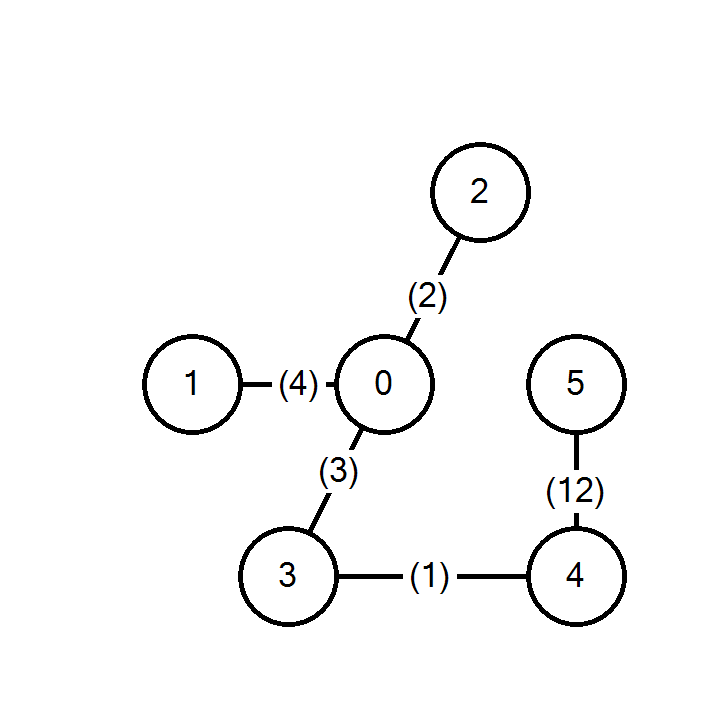
\includegraphics[width=0.4\linewidth]{graf-ej-1}
	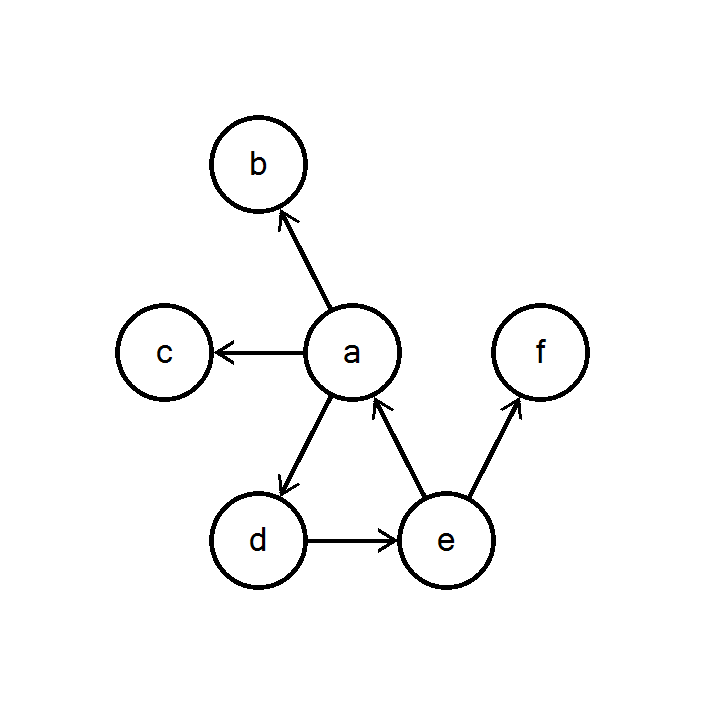
\includegraphics[width=0.4\linewidth]{graf-ej-2}
	\caption{Ejemplo de grafo no dirigido ponderado, izquierda, y grafo dirigido no ponderado, derecha.}
	\label{fig:graf-ej}
\end{figure}

A continuación plantearemos algunas definiciones sobre distintos tipos de grafos.

\begin{definicion}
	Un \textit{grafo finito} es un grafo $G$ (dirigido o no dirigido), con un número finito de vértices, es decir, el conjunto $V$ es finito.
\end{definicion}

\begin{definicion}
	Un \textit{grafo de incidencia finita} es un grafo $G$ donde el grado de incidencia de cada vértice es finito, es decir, $g(v)$ es finito para cada $v\in V$.
\end{definicion}

\begin{definicion}
	Dado un grafo $G=(V,E)$: 
	\begin{itemize}
		\item Se dirá que $G'=(V',E')$ es un \textit{subgrafo} de $G$ si $V'\subseteq V$, $E'\subseteq E$ y dado $\{u,v\}$ en $E'$, $u,v\in V'$.
		\item Se dirá que $G'=(V,E')$ es un \textit{subgrafo parcial} de $G$ si $E'\subseteq E$.
	\end{itemize} 
\end{definicion}

\begin{definicion}
	Dado un grafo $G=(V,E)$ y $B\subseteq V$, se dirá \textit{subgrafo de G inducido por B} a $G_B=(B,E_B)$ con
	$$E_B=\{(i,j)\in E:\ i,j\in B\}$$
	en caso de ser grafo dirigido, y
	$$E_B=\{\{i,j\}\in E:\ i,j\in B\}$$
	en caso de ser no dirigido.
\end{definicion}

Un concepto natural que surge al hablar de grafos es el de camino entre dos nodos, definimos a continuación formalmente el concepto tanto del camino como tal como de la longitud del mismo.

\begin{definicion}
	Dado un grafo $G$, un \textit{camino} es una sucesión de vértices $v_1v_2...v_{n+1}$ y aristas $e_1e_2...e_n$ tales que $e_i=\{v_i,v_{i+1}\}$ si es un grafo no dirigido, o bien $e_i=(v_i,v_{i+1})$ si es un grafo dirigido, $\forall i \in \{1,...,n\}$. Para referirnos a un camino de ahora en adelante, utilizaremos la sucesión de vértices $v_1...v_{n+1}$ si no es necesario conocer las aristas en concreto, o $e_1...e_n$ si necesitamos conocerlas.
\end{definicion}

\begin{definicion}
	Un camino se dirá \textit{simple} si ninguno de sus vértices está repetido en el propio camino, es decir, si pasa por sus vértices una única vez.
\end{definicion}

\begin{definicion}
	Dado un grafo $G$, se define un \textit{ciclo}, sobre el mismo, como un camino en el que el nodo inicial y final son el mismo.
\end{definicion}

\begin{definicion}
	Se define la \textit{longitud} de un camino $v_1v_2...v_{n+1}$ con aristas $e_1e_2...e_n$ como sigue: 
	$$Long(v_1v_2...v_{n+1}) = \sum_{i=1}^{n}\omega(e_i)$$
	En caso de que el grafo no sea ponderado, supondremos coste $1$ para todas las aristas, en cuyo caso, la longitud del camino será $n$.
\end{definicion}

Diremos, en un grafo ponderado, que un ciclo es \textit{negativo}, si la longitud del mismo es negativa.

\begin{definicion}
	Dado un espacio métrico, se define una \textit{geodésica} entre dos puntos del espacio como una línea de mínima longitud que une los puntos.
\end{definicion}

En este trabajo nos centraremos en el estudio de las geodésicas sobre grafos, donde las líneas son caminos. \\

Definimos a continuación una función que nos será útil para poder definir el concepto de geodésica.

\begin{definicion}\label{def:dist}
	Dado un grafo finito $G=(V,E)$ ponderado con pesos estrictamente positivos,  y $v_0,v_1\in V$. Definimos $d:V\times V \rightarrow \mathbb{R}\cup \{\infty\}$ como sigue:
	$$d(v_0,v_1)= \left\{ \begin{array}{lcc}
		min\{Long(v_0...v_1) : v_0...v_1\ camino\ desde\ v_0\ a\ v_1\}, &   si\ existe\ camino\ entre\ v_0\ y\ v_1 \\
		\\ \infty, &  en\ otro\ caso.
	\end{array}
	\right.$$
\end{definicion}

Sabemos que existe el mínimo, pues si no hay ciclos, como los conjuntos de vértices y aristas son finitos, el conjunto de caminos entre dos vértices es también finito. Y, de existir algún ciclo, como no puede ser negativo, repetir el mismo ciclo dentro de un camino aumenta la longitud total, por lo que dichos caminos no pueden ser el mínimo, si nos restringimos a los caminos que no pasan por el ciclo, esta cantidad es finita, al igual que antes. Es decir, en un grafo ponderado con pesos positivos siempre existe una geodésica entre dos puntos cualesquiera. \\

Probaremos a continuación que, tal y como sugiere la definición, $d$ es una distancia.

\begin{proposicion}\label{prop:distancia}
	Sea $G$ un grafo finito no dirigido y ponderado, con pesos estrictamente positivos. Se verifica que $d:V\times V \rightarrow \mathbb{R}\cup \{\infty\}$ con la definición anterior es una distancia en $G$.
\end{proposicion}

\begin{proof}
	Dado que los únicos caminos de longitud $0$ son aquellos en los que no hay aristas, es claro que $d(v_0, v_1) = 0 \Leftrightarrow v_0 = v_1$. La simetría es clara en un grafo no dirigido, pues un camino desde $v_0$ a $v_1$ es también un camino desde $v_1$ a $v_0$, dado que podemos recorrer las aristas en los dos sentidos. Para probar la desigualdad triangular, es decir, $\forall v_0, v_1, v_2 \in V,\ d(v_0,v_1) \leq d(v_0,v_2) + d(v_2,v_1)$, hay que distinguir dos casos, el primero, si no existe ningún camino que conecte $v_0$ con $v_2$ o ningún camino que conecte $v_2$ con $v_1$, en cuyo caso se tendría $d(v_0,v_1)\leq \infty$, por lo que siempre se verifica la desigualdad. En caso contrario, si existieran caminos que conectan $v_0$ con $v_2$ y $v_2$ con $v_1$, respectivamente, sean $c_1$ y $c_2$ caminos con longitud mínima entre $v_0$ y $v_2$, y $v_2$ y $v_1$, el camino $c$ que resulta de unir $c_1$ con $c_2$ es un camino entre $v_0$ y $v_1$ luego, por definición de $d$, se tiene
	$$d(v_0, v_1) \leq Long(c) = Long(c_1)+Long(c_2)=d(v_0,v_2)+d(v_2,v_1)$$
	como se quería.
\end{proof}

\begin{proposicion}
	Sea $G$ un grafo finito dirigido y ponderado, con pesos exclusivamente positivos, se verifica que $d:V\times V \rightarrow \mathbb{R}\cup \{\infty\}$ con la definición anterior es una distancia asimétrica en $G$.
\end{proposicion}

Esta proposición no necesita demostración, pues los argumentos utilizados para probar la no negatividad y la desigualdad triangular en la \autoref{prop:distancia} son válidos también para grafos dirigidos.

\begin{definicion}
	Dado un grafo $G=(V,E)$ y un camino $v_0...v_1$ entre los vértices $v_0$ y $v_1$, a dicho camino se le llama \textit{camino de longitud mínima} desde $v_0$ a $v_1$ si y solo si es la geodésica entre $v_0$ y $v_1$, es decir:
	$$Long(v_0...v_1) = d(v_0, v_1).$$
\end{definicion}

\begin{definicion}
	Dado un grafo $G=(V,E)$ se define el \textit{grafo de caminos de longitud mínima} con raíz $s\in V$ como un subgrafo $G'$ en el que todo camino entre $s$ y cualquier otro nodo $v$ es de longitud mínima, además, existe al menos un camino entre $s$ y cada nodo de $G'$.
\end{definicion}

Veremos a continuación un par de propiedades muy interesantes asociadas a los caminos de longitud mínima.

\begin{proposicion}\label{prop:separa_cam_min_long}
	Dado un camino de longitud mínima $v_0...v_i...v_1$ desde $v_0$ a $v_1$, se verifica:
	\begin{itemize}
		\item $v_0...v_i$ es un camino de longitud mínima desde $v_0$ a $v_i$.
		\item $v_i...v_1$ es un camino de longitud mínima desde $v_i$ a $v_1$.
	\end{itemize}
\end{proposicion}

\begin{proof}
	Sea $e_1...e_{i-1}$ el conjunto de aristas asociadas al camino entre $v_0$ y $v_i$, entonces, por contradicción, supongamos que $v_0...v_i$ no es un camino de longitud mínima (el caso en que $v_i...v_1$ no es un camino de longitud mínima es análogo), al no ser camino de longitud mínima, debe existir otro camino entre $v_0$ y $v_i$ de longitud menor, es decir, $\exists e_1'...e_m'$ camino entre $v_0$ y $v_i$ con $Long(e_1'...e_m') < Long(e_1...e_{i-1})$. Llamemos $e_i...e_n$ al conjunto de aristas del camino entre $v_i$ y $v_1$, entonces, juntando el nuevo camino entre $v_0$ y $v_i$ con éste último, obtenemos:
	\begin{equation}
		\begin{split}
			Long(e_1'...e_m'e_i...e_n) & =Long(e_1'...e_m') + Long(e_i...e_n) \\
			& < Long(e_1...e_{i-1}) + Long(e_i...e_n) \\
			& =	Long(e_1...e_n)
		\end{split}
	\end{equation}
	Esto es una contradicción pues, por hipótesis, $Long(e_1...e_n) = d(v_0,v_1)$, al ser $e_1...e_n$ camino de longitud mínima, pero hemos encontrado entonces un camino entre $v_0$ y $v_1$, el cual es $e_1'...e_m'e_i...e_n$, de longitud menor, lo que no puede ser.
\end{proof}

\begin{proposicion}
	Sea $G=(V,E,\omega)$ un grafo de incidencia finita ponderado con pesos positivos tal que:
	\begin{itemize}
		\item $\omega (e)\geq a>0\ \ \ \forall e\in E.$
	\end{itemize}
	Entonces, si existe un camino entre dos nodos, existe un camino de longitud mínima entre ambos (geodésica).
\end{proposicion}

\begin{proof}
	Sean $v_0,v_1\in V$ tales que existe un camino de longitud $L>0$ entre ambos, si $c$ es otro camino entre $v_0$ y $v_1$ de $K$ aristas, entonces
	$$Long(c) \geq Ka$$
	por hipótesis.\\
	Si $Ka>L$, $c$ no puede ser una geodésica, consideramos entonces el subgrafo inducido por los vértices que se pueden unir con $v_0$ mediante caminos de $K\leq \frac{L}{a}$ lados. El vértice $v_1$ pertenece a dicho grafo por el camino inicial. Ahora, por ser $G$ un grafo de incidencia finita, se tiene que dicho subgrafo es finito y, por tanto, existe una geodésica que une $v_0$ con $v_1$ en el subgrafo y, dado que el resto de caminos $c$ entre $v_0$ y $v_1$ tienen longitud $Long(c) > L$, la geodésica en el subgrafo es geodésica también en G.
\end{proof}

\begin{proposicion}
	Todo camino de longitud mínima sobre un grafo sin ciclos negativos es simple.
\end{proposicion}

\begin{proof}
	Supongamos que existe un camino de longitud mínima no simple, es decir, que pasa por uno de sus vértices al menos dos veces. El camino que va desde este vértice al mismo es un ciclo y, al no existir ciclos negativos, eliminando dicho ciclo del camino original, obtenemos otro camino de longitud menor, contradiciendo el hecho de que era un camino de longitud mínima.
\end{proof}

Para trabajar con grafos, necesitamos representarlos de alguna manera, para ello se definen a continuación dos estructuras muy utilizadas a la hora de la representación de grafos:

\begin{definicion}
	Dado un grafo finito $G$, con $|V|=n$, llamaremos \textit{matriz de adyacencia} de $G$ a una matriz $A_{n\times n}=(a_{ij})$ de tal manera que:
	$$a_{ij}= \left\{ \begin{array}{lcc}
		1 &   si\ (v_i,v_j)\in E\ (\{v_i,v_j\}\in E) \\
		\\ 0 &  en\ otro\ caso
	\end{array}
	\right.$$
\end{definicion}

\begin{definicion}
	Dado un grafo finito $G$, con $|V|=n$, se define la \textit{lista de adyacencia} de $v \in V$ como:
	$$Adj(v) = \{u \in V : (v,u)\in E\ (\{v,u\}\in E)\}$$
	De tal manera que para representar el grafo, basta calcular la lista de adyacencia de cada vértice.
\end{definicion}

\section{Propiedades de los caminos de longitud mínima y la relajación de aristas}\label{sec:2.2}

Las propiedades que vamos a mencionar en esta sección junto a la operación de relajación de una arista han sido extraídas del capítulo 24 de la referencia \cite{algorithms}. \\

Estas propiedades junto con la operación de relajación de una arista serán útiles para probar la corrección de los algoritmos que trabajan con aristas de pesos negativos, para los cuales la función $d$ definida en \autoref{def:dist} no nos sirve, por ello, definimos la función $d:V\times V \rightarrow \mathbb{R}\cup \{\infty,-\infty\}$ como sigue:
$$d(v_0,v_1)= \left\{ \begin{array}{lcc}
	-\infty & si\ existe\ un\ camino\ entre\ v_0\ y\ v_1,\ y\ este\\ & se\ puede\ conectar\ con\ un\ ciclo\ negativo
	\\ min\{Long(v_0...v_1) : v_0...v_1\ camino\} &   si\ existen\ caminos\ entre\ v_0\ y\ v_1,\ y\ ninguno\\ & se\ puede\ conectar\ con\ un\ ciclo\ negativo
	\\ \infty &  en\ otro\ caso
\end{array}
\right.$$ \\

A continuación explicaremos la operación de \textit{relajación de una arista}, la cual utiliza el coste actual de los vértices. Dicho coste representa el valor de la longitud del camino de menor longitud desde el inicio hasta el vértice correspondiente que ha calculado hasta el momento algún algoritmo. \\

La \textit{relajación de una arista} consiste en, dada una arista $(u,v)$, si el coste actual de $v$ es mayor que el coste actual de $u$ más el peso de la arista, se modifica el coste actual de $v$ a la nueva cantidad y se establece a $u$ como el padre de $v$, si el coste fuera igual, simplemente se añade $u$ a los padres de $v$. \\

Desde un punto de vista algorítmico, el pseudocódigo asociado a dicha operación es el siguiente:

\begin{breakablealgorithm}
	\caption{Relajar(u, v)}
	\begin{algorithmic}[1]
		\If{$v.d > u.d + d[u][v]$}
			\State $v.d = u.d + d[u][v]$
			\State $v.p = \{u\}$
		\ElsIf{$v.d == u.d + d[u][v]$}
			\If{$!v.p.contains(u)$}
				\State $v.p.push(u)$
			\EndIf
		\EndIf
	\end{algorithmic}
\end{breakablealgorithm}

En el algoritmo anterior, $u$ y $v$ son los vértices que forma la arista $(u,v)$ y el peso de las aristas viene dado por la matriz $d$, la distancia actual de un vértice viene dada por $v.d$ y la lista de padres viene dada por $v.p$. El condicional de la línea $5$ sirve para evitar que se repita el mismo camino varias veces.\\

Además de esta operación, necesitaremos inicializar el grafo con unos valores de distancia y una lista de padres inicial para cada vértice, para ello ponemos como distancia inicial $\infty$ y lista de padres nula, luego simplemente establecemos la distancia del nodo inicial a $0$. El pseudocódigo que recoge este proceso es el siguiente:

\begin{breakablealgorithm}
	\caption{Inicializacion(G, s)}
	\begin{algorithmic}[1]
		\For{$v \in G.V$}
			\State $v.d = \infty$
			\State $v.p = \{\}$
		\EndFor
		\State $s.d = 0$
	\end{algorithmic}
\end{breakablealgorithm}

Donde $G$ es el grafo, $s$ el nodo inicial, la distancia actual de un vértice viene dada por $v.d$ y la lista de padres viene dada por $v.p$. \\

\subsection{Propiedades}

\begin{lema}\label{lema:des_tri}
	\textbf{(Desigualdad Triangular)} Sea $G=(V,E)$ un grafo con función de pesos $\omega : E\rightarrow \mathbb{R}$ y sea $s\in V$ el vértice inicial. Entonces, para todas las aristas $(u,v)\in E$, se tiene
	$$d(s,v)\leq d(s,u)+\omega (u,v).$$
\end{lema}

\begin{proof}
	Sea $p$ el camino de longitud mínima entre $s$ y $v$, por definición de $d$, como el camino que resulta de unir el camino de longitud mínima entre $s$ y $u$ con la arista $(u,v)$ es un camino entre $s$ y $v$, debe tener mayor longitud que $p$, pues este es el camino de menor longitud.
\end{proof}

\begin{lema}\label{lema:lim_sup}
	\textbf{(Propiedad del límite superior)} Sea $G=(V,E)$ un grafo con función de pesos $\omega : E\rightarrow \mathbb{R}$. Sea $s\in V$ el vértice inicial y supongamos que el grafo ha sido inicializado por $Inicializacion(G,s)$. Entonces, $v.d \geq d(s,v)\ \forall v\in V$ y esta propiedad se mantiene bajo cualquier secuencia de relajaciones de las aristas de $G$. De hecho, una vez $v.d$ alcanza su límite inferior $d(s,v)$, éste nunca cambia.
\end{lema}

\begin{proof}
	Probamos la propiedad $v.d \geq d(s,v) \forall v\in V$ por inducción sobre el número de relajaciones. \\
	Para el paso base, tras la inicialización, $v.d \geq d(s,v)$ es cierto pues $v.d = \infty\ \forall v\in V-\{s\}$ y $s.d=0\geq d(s,s)$ (nótese que $d(s,s)=-\infty$ si $s$ es parte de un ciclo negativo, o $0$ en otro caso). \\
	Ahora, en el paso de inducción, consideremos la relajación de la arista $(u,v)$. Por hipótesis de inducción, $x.d\geq d(s,x)\ \forall x\in V$ antes de la relajación. El único valor de $d$ que puede variar en la relajación es $v.d$ y, si este cambia, se verifica
	\begin{align*}
			v.d & =u.d + \omega(u,v) \\
			& \geq d(s,u) + \omega(u,v) & (\textrm{hipótesis de inducción}) \\
			& \geq d(s,v) & (\textrm{desigualdad triangular (\autoref{lema:des_tri})})
	\end{align*}
	Para ver que el valor de $v.d$ nunca cambia cuando $v.d=d(s,v)$, basta ver que $v.d$ no puede decrecer, pues acabamos de probar que $v.d\geq d(s,v)$ y tampoco puede aumentar pues la relajación no aumenta los valores de $d$.
\end{proof}

\begin{corolario}\label{cor:no_path}
	\textbf{(Propiedad de no camino)} Sea $G=(V,E)$ un grafo con función de pesos $\omega : E\rightarrow \mathbb{R}$. Sea $s\in V$ el nodo inicial y $v\in V$ otro nodo tal que no existe ningún camino entre $s$ y $v$, entonces, tras inicializar el grafo con $Inicializacion(G,s)$, se tiene $v.d=d(s,v)=\infty$ y esta igualdad se mantiene a través de cualquier relajación de aristas.
\end{corolario}

\begin{proof}
	Por la propiedad del límite superior (\autoref{lema:lim_sup}), $\infty=d(s,v)\leq v.d$ y, por tanto, $v.d=\infty =d(s,v).$
\end{proof}

\begin{lema}\label{lema:2.3}
	Sea $G=(V,E)$ un grafo con función de pesos $\omega : E\rightarrow \mathbb{R}$, y sea $(u,v)\in E$. Entonces, inmediatamente después de relajar la arista $(u,v)$, se tiene $v.d\leq u.d + \omega(u,v)$.
\end{lema}

\begin{proof}
	Si, justo antes de relajar la arista $(u,v)$ se tiene $v.d > u.d + \omega(u,v)$, entonces $v.d = u.d + \omega(u,v)$ tras relajar. Si, por el contrario, $v.d\leq u.d + \omega(u,v)$ justo antes de relajar, entonces no cambian ni $u.d$ ni $v.d$, por lo que se tiene $v.d\leq u.d + \omega(u,v)$ justo después.
\end{proof}

\begin{observacion}
	Cuando escribamos $s \leadsto u \rightarrow v$, nos estaremos refiriendo a un camino entre $s$ y $v$, tal que el penúltimo nodo del camino es $u$.
\end{observacion}

\begin{lema}\label{lema:convergencia}
	\textbf{(Propiedad de convergencia)} Sea $G=(V,E)$ un grafo con función de pesos $\omega : E\rightarrow \mathbb{R}$, sea $s\in V$ el nodo inicial y supongamos que $s \leadsto u \rightarrow v$ es un camino de mínima longitud para algunos vértices $u,v\in V$. Supongamos que se inicializa el grafo con $Inicializacion(G,s)$, y que una serie de pasos de relajación incluye la relajación de la arista $(u,v)$. Entonces, si $u.d=d(s,u)$ en algún momento anterior a la relajación de la arista, $v.d=d(s,v)$ en todo momento tras la relajación.
\end{lema}

\begin{proof}
	Por la propiedad del límite superior (\autoref{lema:lim_sup}), si $u.d=d(s,u)$ en algún momento anterior a la relajación de la arista, la igualdad se mantiene en todo momento. En particular, tras relajar la arista, se tiene:
	\begin{align*}
			v.d & \leq u.d + \omega(u,v) & (\textrm{\autoref{lema:2.3}}) \\
			& = d(s,u) + \omega(u,v) \\
			& = d(s,v) &(\textrm{\autoref{prop:separa_cam_min_long}})
	\end{align*}
	Por la propiedad del límite superior (\autoref{lema:lim_sup}), $v.d\geq d(s,v)$, de lo que concluimos $v.d = d(s,v)$, y esta igualdad se mantiene en adelante.
\end{proof}

\begin{lema}\label{lema:relaj_caminos}
	\textbf{(Propiedad de relajación de caminos)} Sea $G=(V,E)$ un grafo con función de pesos $\omega : E\rightarrow \mathbb{R}$ y sea $s\in V$ el nodo inicial. Consideremos cualquier camino de longitud mínima $p = v_0v_1...v_k$ desde $s=v_0$ a $v_k$. Si $G$ es inicializado con $Inicializacion(G,s)$ y ocurre una secuencia de relajación de aristas que incluye, en orden, la relajación de las aristas $(v_0,v_1),(v_1,v_2),...,(v_{k-1},v_k)$, entonces $v_k.d=d(s,v_k)$ tras esta secuencia y en todo momento posterior. Esta propiedad se mantiene sin importar el resto de relajaciones que sucedan durante la secuencia, incluso si están mezcladas con la relajación de las aristas de $p$.
\end{lema}

\begin{proof}
	Probamos por inducción que tras la relajación de la $i$-ésima arista del camino $p$, se tiene $v_i.d=d(s,v_i)$. Para el paso base, $i=0$, y antes de que ninguna arista de $p$ sea relajada, por la inicialización tenemos que $v_0.d=s.d=0=d(s,s)$. Por la propiedad del límite superior (\autoref{lema:lim_sup}), el valor de $s.d$ nunca cambia tras su inicialización. \\
	Para el paso de inducción, asumimos que $v_{i-1}.d=d(s,v_{i-1})$ y comprobamos el resultado de aplicar la relajación de la arista $(v_{i-1},v_i)$. Por la propiedad de convergencia (\autoref{lema:convergencia}), tras relajar dicha arista, tenemos $v_i.d=d(s,v_i)$, y esta igualdad se mantiene en todo momento desde entonces.
\end{proof}

Para la siguiente propiedad debemos introducir primero un concepto que nos vendrá muy bien a la hora de analizar algoritmos sobre grafos.

\begin{definicion}
	Dado un grafo $G=(V,E)$ en el que, tras aplicar un algoritmo con nodo inicial $s$, se han almacenado los predecesores de cada nodo como $v.p$, se define el \textit{subgrafo de predecesores} $G_{\pi}$ como el subgrafo de $G$ donde
	$$V_{\pi}=\{v\in V : v.p \neq NIL\}\cup \{s\}$$
	$$E_{\pi}=\{(v.p,v)\in E : v\in V_{\pi}-\{s\}\}$$
\end{definicion}

\begin{proposicion}\label{prop:subg_pred}
	\textbf{(Propiedad del subgrafo de predecesores)} Sea $G=(V,E)$ un grafo con función de pesos $\omega : E\rightarrow \mathbb{R}$, sea $s\in V$ el nodo inicial y supongamos que $G$ no contiene ciclos negativos alcanzables desde $s$. Tras inicializar el grafo con $Inicializacion(G,s)$ y ejecutar cualquier secuencia de relajaciones que produzca $v.d=d(s,v)\ \forall v\in V$, el grafo de predecesores $G_{\pi}$ es un grafo de caminos de longitud mínima con raíz $s$.
\end{proposicion}

\begin{proof}
	Primero, es claro que todos los vértices del grafo $G_{\pi}$ son alcanzables desde $s$, pues, por definición, $V_{\pi}$ son los vértices que tienen al menos un predecesor, pues los vértices alcanzables en un grafo son aquellos con $d(s,v) = v.d$ finita, y un nodo tiene valor $d$ finito si tiene predecesor. \\
	Ahora debemos probar que todo camino desde $s$ es un camino de longitud mínima. Sea $p=v_0v_1...v_k$ con $v_0=s$ y $v_k=v$ un camino de longitud mínima desde $s$ hasta $v\in V$, se tiene para $i=1,...,k$, que $v_i.d=d(s,v_i)$ y que $v_i.d \geq v_{i-1}.d + \omega(v_{i-1},v_i)$, de lo que concluimos $\omega(v_{i-1},v_i) \leq d(s,v_i)-d(s,v_{i-1})$. Sumando todos los pesos a lo largo del camino $p$ obtenemos
	\begin{align*}
		\omega(p) & = \sum_{i=1}^{k}\omega(v_{i-1},v_i) \\
		& \leq \sum_{i=1}^{k}(d(s,v_i)-d(s,v_{i-1})) \\
		& = d(s,v_k) - d(s,v_0) &(\textrm{Los sumandos se cancelan}) \\
		& = d(s,v_k) & (d(s,v_0)=d(s,s)=0)
	\end{align*}
	Por lo que, $\omega(p)\leq d(s,v_k)$. Puesto que $d(s,v_k)$ es un límite inferior del peso de cualquier camino de $s$ a $v_k$, concluimos que $\omega(p)= d(s,v_k)$ y, por tanto, $p$ es camino de longitud mínima.
\end{proof}

\endinput


% !TeX root = ../libro.tex
% !TeX encoding = utf8

\setchapterpreamble[c][0.75\linewidth]{%
	\sffamily
	En este capítulo abordaremos algunos algoritmos de búsqueda en grafos, con el objetivo de encontrar caminos entre puntos, geodésicas y componentes conexas asociadas a los distintos grafos. En esta sección nos referiremos a los vértices del grafo por nodos.
	\par\bigskip
}
\chapter{Algoritmos de búsqueda en grafos}\label{ch:tercer-capitulo}

\section{Algoritmo de búsqueda en anchura}

El algoritmo de búsqueda en anchura (BFS-Breadth First Search en inglés) es un algoritmo de búsqueda no informada, es decir, que cuando se da un paso en el algoritmo, no se sabe si este es el mejor posible. Es uno de los algoritmos más simples de búsqueda en grafos y funciona como base para el desarrollo de otros algoritmos más complejos. La idea intuitiva del algoritmo es partir del nodo inicial e ir explorando todos los nodos vecinos (conectados mediante un camino), cuando se han explorado todos los vecinos, se repite el proceso para cada uno de estos, hasta recorrer todo el grafo. \\

El nombre de búsqueda en anchura viene del hecho de que el algoritmo explora la frontera entre nodos explorados y no explorados, de manera uniforme a lo largo del ancho de la misma, es decir, explora todos los nodos a distancia $k$ antes de explorar un nodo a distancia $k+1$. \\

El algoritmo funciona tanto en grafos no dirigidos como grafos dirigidos, sin embargo, requiere que los pesos de las aristas sean $1$, es decir, que sea un grafo no ponderado. El algoritmo se puede utilizar tanto para calcular las componentes conexas de un grafo como para encontrar los caminos de mínima longitud, geodésicas, entre dos nodos. \\

Desde un punto de vista matemático, sea $p$ el nodo inicial, el algoritmo consiste en explorar la bola cerrada $\overline B_p(r)$ empezando en $r=1$, marcando los elementos dentro de la bola, e ir aumentando en cada paso el radio en una unidad hasta que no se puedan alcanzar más elementos desde el nodo inicial, es decir, hasta que $\overline B_p(r)\cap \overline B_p(r+1) = \emptyset$. Para el cálculo de componentes conexas, si, tras terminar el proceso anterior, quedan nodos sin explorar, se selecciona un nodo no explorado y se repite el proceso, hasta que todos los nodos sean explorados. Para el cálculo de las geodésicas la exploración continúa hasta encontrar el nodo destino, si no se encuentra, no existe camino entre los nodos.

\begin{proposicion}\label{prop:BFS}
	\textbf{(Corrección del algoritmo de búsqueda en anchura)} Sea $v \in V$ el nodo inicial y $p \in V$ el nodo final, el camino encontrado por el algoritmo de búsqueda en anchura entre estos nodos es una geodésica.
\end{proposicion}

\begin{proof}
	Sea $l$ la longitud del camino encontrado, por construcción del algoritmo, esto supone dos cosas, por un lado, $p \in \overline B_v(l)$, y, por otro lado, $p \notin \overline B_v(r)\ \forall r<l$ pues, de lo contrario, el algoritmo hubiera parado antes de explorar $\overline B_v(l)$ y la longitud sería menor. Pero entonces esto supone que no existe ningún camino entre $v$ y $p$ de longitud menor que $l$, es decir, que el camino encontrado de longitud $l$ es una geodésica, como se quería.
\end{proof}


\begin{figure}[htb]
	\centering
	\begin{subfigure}{0.25\linewidth}
		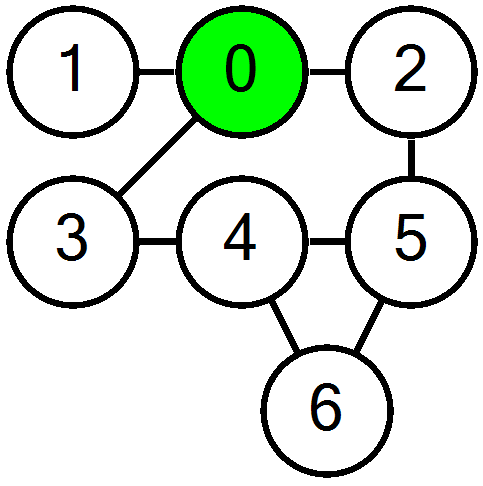
\includegraphics[width=\linewidth]{BFS/graf-bfs-camino-1}
		\caption{}
	\end{subfigure}
	\begin{subfigure}{0.25\linewidth}
		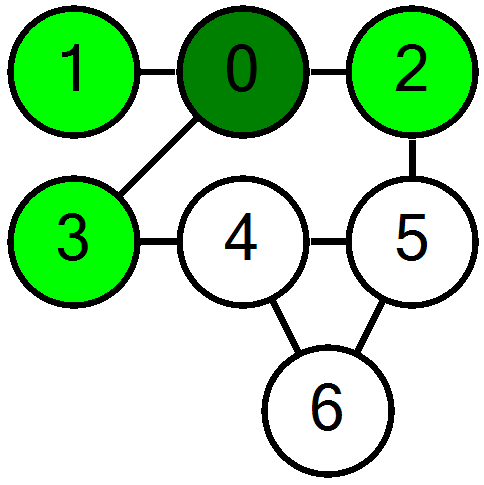
\includegraphics[width=\linewidth]{BFS/graf-bfs-camino-2}
		\caption{}
	\end{subfigure}
	\begin{subfigure}{0.25\linewidth}
		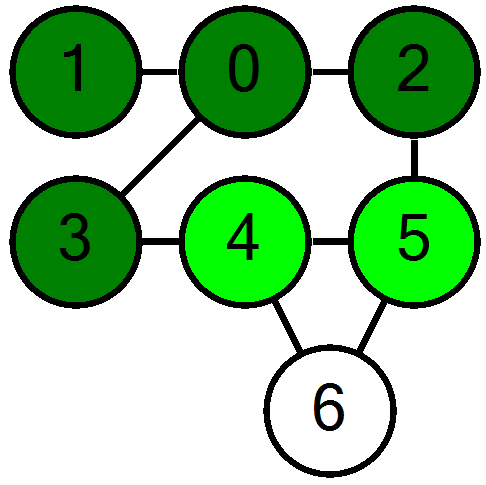
\includegraphics[width=\linewidth]{BFS/graf-bfs-camino-3}
		\caption{}
	\end{subfigure}
	\begin{subfigure}{0.25\linewidth}
		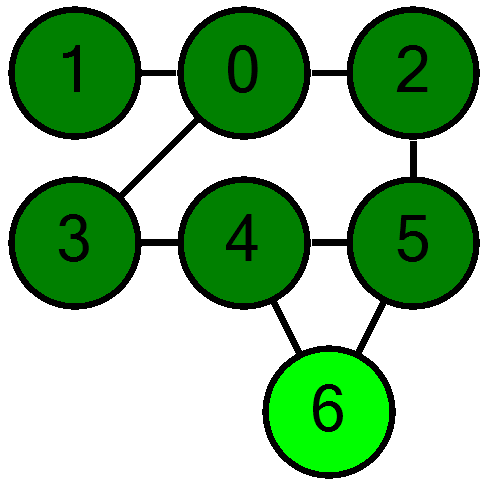
\includegraphics[width=\linewidth]{BFS/graf-bfs-camino-4}
		\caption{}
	\end{subfigure}
	\begin{subfigure}{0.25\linewidth}
		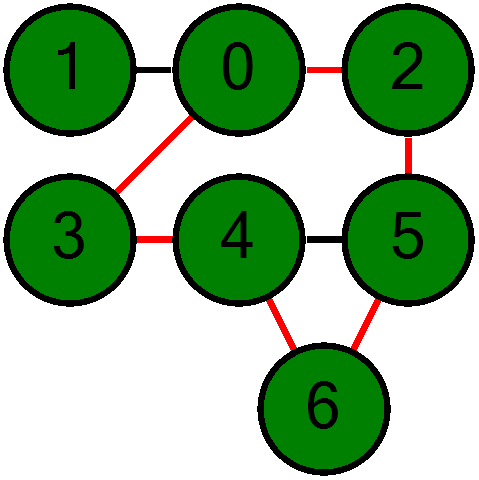
\includegraphics[width=\linewidth]{BFS/graf-bfs-camino-5}
		\caption{}
	\end{subfigure}
	\caption{Cálculo de las geodésicas entre el nodo $0$ y el nodo $6$.}
	\label{fig:bfs-camino}
\end{figure}

\begin{figure}[!]
	\centering
	\begin{subfigure}{0.25\linewidth}
		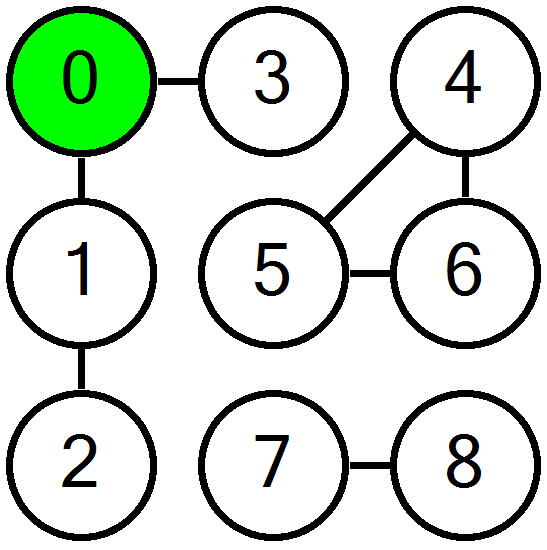
\includegraphics[width=\linewidth]{BFS/graf-bfs-conexas-1}
		\caption{}
	\end{subfigure}
	\begin{subfigure}{0.25\linewidth}
		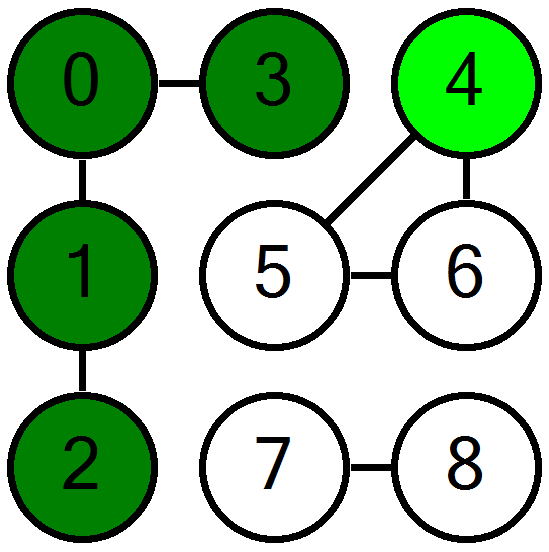
\includegraphics[width=\linewidth]{BFS/graf-bfs-conexas-2}
		\caption{}
	\end{subfigure}
	\begin{subfigure}{0.25\linewidth}
		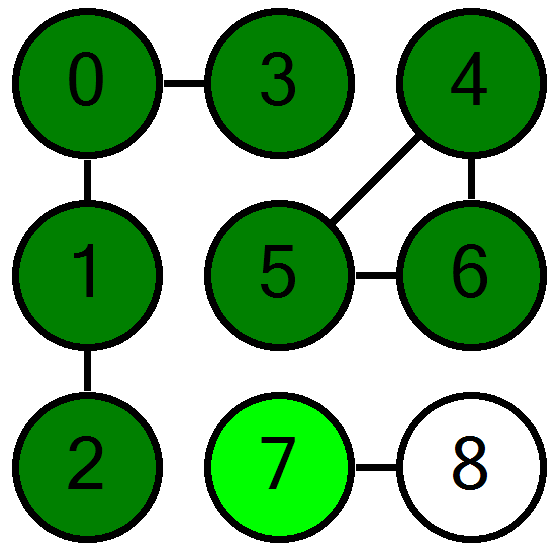
\includegraphics[width=\linewidth]{BFS/graf-bfs-conexas-3}
		\caption{}
	\end{subfigure}
	\begin{subfigure}{0.25\linewidth}
		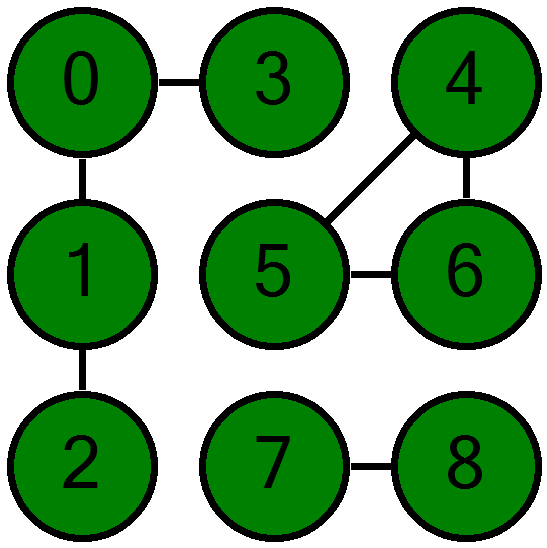
\includegraphics[width=\linewidth]{BFS/graf-bfs-conexas-4}
		\caption{}
	\end{subfigure}
	\caption{Cálculo de las componentes conexas del grafo, en este caso, 3.}
	\label{fig:bfs-conexas}
\end{figure}

En la \autoref{fig:bfs-camino} y la \autoref{fig:bfs-conexas} podemos observar un ejemplo del comportamiento del algoritmo, tanto para encontrar las geodésicas entre dos nodos como para calcular el número de componentes conexas. En el primer caso, se muestra en cada figura el estado de los nodos tras la exploración completa de cada bola, marcando en verde oscuro los nodos explorados y en verde pistacho los nodos visitados que serán explorados en la siguiente bola, por ejemplo, en el apartado (c) acaba de finalizar la exploración de la bola $\overline B_0(1)$. En la segundo figura se muestra el estado del grafo tras finalizar el algoritmo base sobre cada componente, y haber seleccionado el siguiente nodo a explorar.


\subsection{Implementación del algoritmo de búsqueda en anchura}
A continuación veremos la implementación mediante pseudocódigo de las dos versiones del algoritmo que trabajaremos, la primera, cuya finalidad será la de encontrar todas las geodésicas entre dos nodos, y la segunda, que calculará el número de componentes conexas del grafo. \\

Para la construcción del algoritmo, utilizaremos la representación mediante listas de adyacencia. \\

Empezamos por el algoritmo de cálculo de geodésicas entre dos nodos.

\begin{algorithm}
	\caption{BFS\_geodesicas(G, v, p)}
	\begin{algorithmic}[1]
		\For{$u \in G.V$}
			\State $u.explorado = False$
			\State $u.distancia = \infty$
			\State $u.predecesor = \{\}$
		\EndFor
		\State $v.distancia = 0$
		\State $Cola\ Q = \emptyset$
		\State $Q.push(v)$
		\While{$Q \neq \emptyset$}
			\State $u = Q.pull()$
			\If{$u == p$}
				\Return $TRUE$
			\EndIf
			\For{$n \in G.Adj[u]$}
				\If{$!n.explorado$}
					\If{$n.distancia >= u.distancia + 1$}
						\State $n.distancia = u.distancia + 1$
						\State $n.predecesor.push(u)$
						\State $Q.push(n)$
					\EndIf
				\EndIf
			\EndFor
			\State $u.explorado = True$
		\EndWhile
		\Return $FALSE$
	\end{algorithmic}
\end{algorithm}

En el algoritmo anterior, $G$ es el grafo, $v$ el nodo inicial, $p$ el nodo final y $Q$ es una cola. \\

Esta versión del algoritmo es muy similar a la versión normal del algoritmo, con la excepción de que, para poder encontrar todas las geodésicas, debemos considerar nodos ya visitados, pues pueden ser explorados por varios nodos a la misma distancia. Para evitar que antes de explorar un nodo sea visitado y, por tanto, alterado, por otro nodo a distancia mayor que la primera vez que fue visitado, se ha incluido el condicional de la línea 13, nótese que, al iniciar las distancias a infinito, la primera vez que se visita un nodo, este condicional es siempre cierto. \\

Pasamos a continuación con la versión del algoritmo que calcula el número de componentes conexas del grafo.

\begin{breakablealgorithm}
	\caption{BFS\_conexas(G)}
	\begin{algorithmic}[1]
		\State $N = \emptyset$
		\State $conexas = 0$
		\For{$u \in G.V$}
			\State $u.explorado = False$
			\State $N.push(u)$
		\EndFor
		\While{$N \neq \emptyset$}
			\State $conexas = conexas + 1$
			\State $u = N.pull()$
			\State $u.explorado = True$
			\State $Cola\ Q = \emptyset$
			\State $Q.push(u)$		
			\While{$Q \neq \emptyset$}
				\State $u = Q.pull()$
				\For{$n \in G.Adj[u]$}
					\If{$!n.explorado$}
						\State $Q.push(n)$
						\State $n.explorado = True$
						\State $N.remove(n)$
					\EndIf
				\EndFor
			\EndWhile
		\EndWhile
		\Return $conexas$
	\end{algorithmic}
\end{breakablealgorithm}

Para asegurarnos de que se exploran todos los nodos, los incluimos primero en un conjunto, del que los sacamos conforme los exploramos, y continuamos explorando hasta que dicho conjunto sea vacío. Puesto que, para el cálculo de las componentes conexas tan solo necesitamos conocer si podemos alcanzar un nodo desde el inicio, marcamos como explorado los nodos en la adyacencia del nodo que estamos explorando, de tal manera nos aseguramos que solo entra a la cola una vez. 

\section{Algoritmo de Dijkstra}

El siguiente algoritmo que vamos a estudiar es el algoritmo de Dijkstra, al igual que la búsqueda en anchura, es un algoritmo de búsqueda del camino más corto entre nodos, con la salvedad de que funciona también para grafos ponderados. Su nombre proviene del científico Edsger Dijkstra, que lo ideó en 1956 y publicó por primera vez en 1959. \\

La idea del algoritmo es en esencia, la misma que la búsqueda en anchura, con la salvedad de que la exploración de los nodos se realiza de forma ordenada, es decir, en cada paso, se escoge el nodo que esté a distancia menor de todos los que han sido visitados, para explorar. Al igual que el algoritmo de búsqueda en anchura, este algoritmo no funciona si existen aristas con pesos negativos. \\

A nivel de espacios métricos, sea $p$ el nodo inicial, el primer paso es calcular el mínimo de las distancias del resto de nodos a $p$, sea $r$ dicha distancia, entonces procederemos a explorar la bola cerrada $\overline B_p(r)$, en dicha bola se encuentran el nodo inicial y, al menos, un nodo más, que está a distancia r. El siguiente paso es calcular $r'$, que va a ser el mínimo entre las distancias de los nodos no explorados a $p$, y las distancias de los nodos no explorados a los nodos del conjunto $\overline B_p(r)\backslash\{p\}$ más la distancia de dichos nodos a $p$, es decir:

$$r' = min\{d(p,v):\ v \in V\backslash\overline B_p(r),\ d(p,v) + d(v,u):\ v \in \overline B_p(r)\backslash\{p\},\ u \in V\backslash\overline B_p(r)\}$$

A continuación se explora la bola cerrada $\overline B_p(r')$ y el proceso se repite hasta encontrar el nodo destino.

\begin{proposicion}\label{prop:DJK}
	\textbf{(Corrección del algoritmo de Dijkstra)}Sea $v \in V$ el nodo inicial y $p \in V$ el nodo final, el camino encontrado por el algoritmo de Dijkstra entre estos nodos es una geodésica.
\end{proposicion}

\begin{proof}
	Puesto que $d(p,v) > r,\ v \in V\backslash\overline B_p(r)$, por elección de $r$, y $d(p,v) + d(v,u) > r,\ v \in \overline B_p(r)\backslash\{p\},\ u \in V\backslash\overline B_p(r)$, pues, de lo contrario, $d(p,u) \leq d(p,v) + d(v,u) \leq r$, pero esto significa que $u \in \overline B_p(r)$, lo que es una contradicción. Por tanto, se verifica que, en cada paso del algoritmo, $r' > r$, es decir, que la distancia de los nodos explorados es siempre creciente, por lo que la demostración de la \autoref{prop:BFS} es cierta también para este algoritmo.
\end{proof}

\subsection{Implementación del algoritmo de Dijkstra}

A nivel de implementación el algoritmo difiere un poco de la definición matemática, pues es muy ineficiente tener que actualizar el radio en cada paso, teniendo en cuenta además todos los nodos del grafo. Por esto, se introduce el concepto de nodos \textit{visitados}, que son los nodos vecinos de un nodo explorado, es decir, nodos en la frontera del conjunto de nodos explorados. Se introduce este concepto pues, tras la exploración de un nodo, el siguiente nodo que escoge el algoritmo es el de menor distancia y éste es siempre un nodo en la frontera, es decir, un nodo marcado como visitado, pues el resto de nodos del grafo están a mayor distancia de los nodos en la frontera, ya que los pesos de las aristas son positivos. \\

El procedimiento del algoritmo entonces consiste en explorar el nodo visitado a menor distancia del nodo inicial. La exploración del nodo consiste en marcar todos los nodos vecinos no explorados como visitados y actualizar su distancia al nodo inicial a partir del peso de la arista que los une y la distancia del propio nodo. \\

Este procedimiento mantiene invariante la propiedad principal del algoritmo, la distancia de los nodos explorados es siempre creciente a medida que avanza el algoritmo, lo que permite mantener la corrección del algoritmo probada en la \autoref{prop:DJK}, es decir, lo caminos encontrados de esta manera son geodésicas. \\

\begin{figure}[htb]
	\centering
	\begin{subfigure}{0.32\linewidth}
		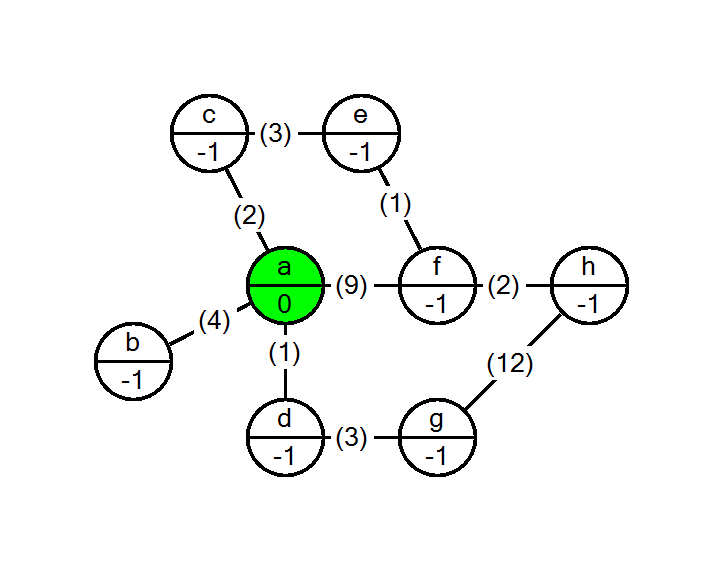
\includegraphics[width=\linewidth]{DJK/graf-djk-1}
		\caption{}
	\end{subfigure}
	\begin{subfigure}{0.32\linewidth}
		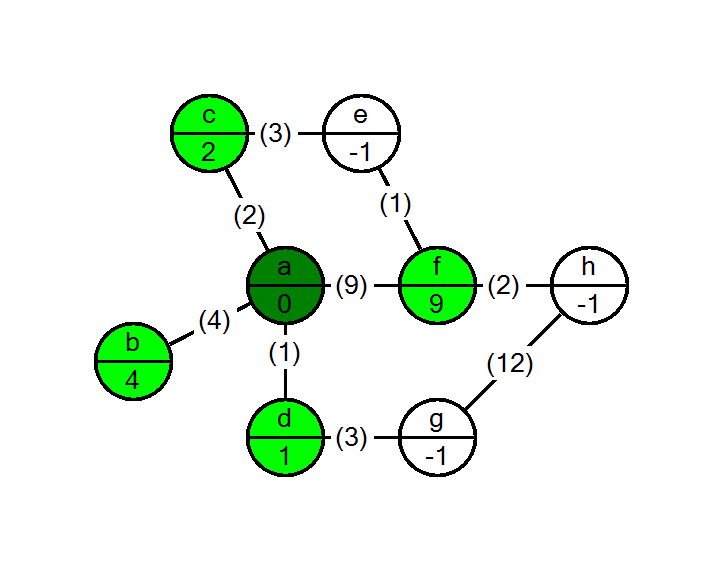
\includegraphics[width=\linewidth]{DJK/graf-djk-2}
		\caption{}
	\end{subfigure}
	\begin{subfigure}{0.32\linewidth}
		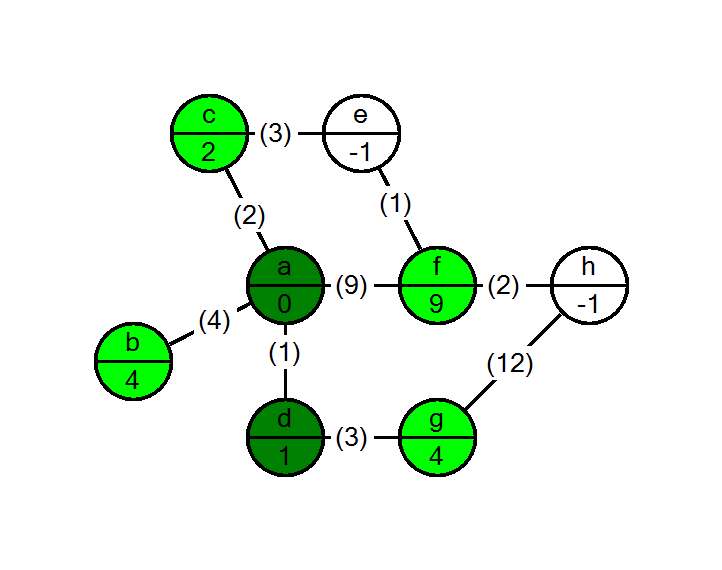
\includegraphics[width=\linewidth]{DJK/graf-djk-3}
		\caption{}
	\end{subfigure}
	\begin{subfigure}{0.32\linewidth}
		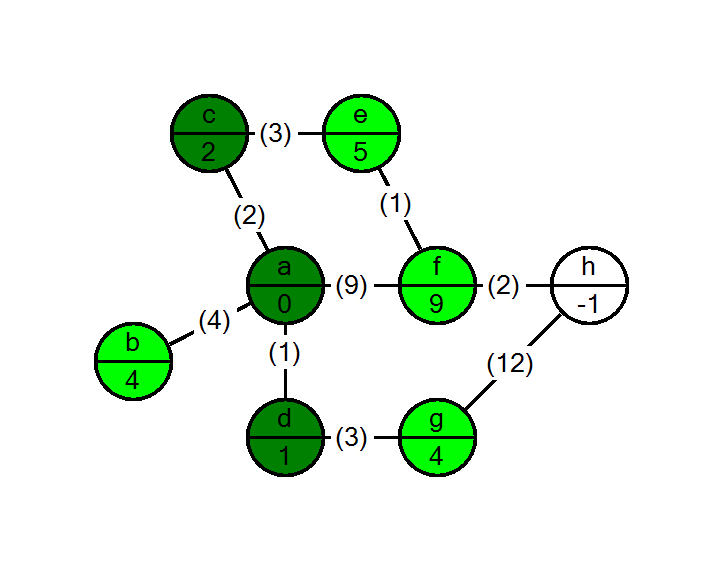
\includegraphics[width=\linewidth]{DJK/graf-djk-4}
		\caption{}
	\end{subfigure}
	\begin{subfigure}{0.32\linewidth}
		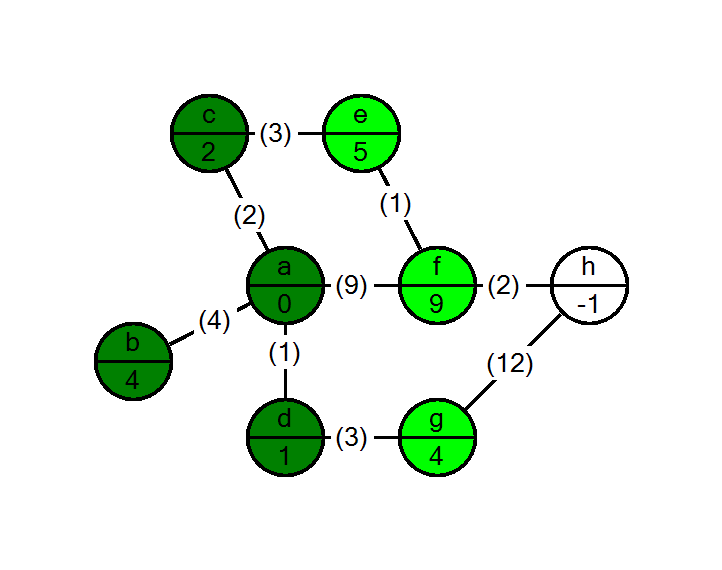
\includegraphics[width=\linewidth]{DJK/graf-djk-5}
		\caption{}
	\end{subfigure}
	\begin{subfigure}{0.32\linewidth}
		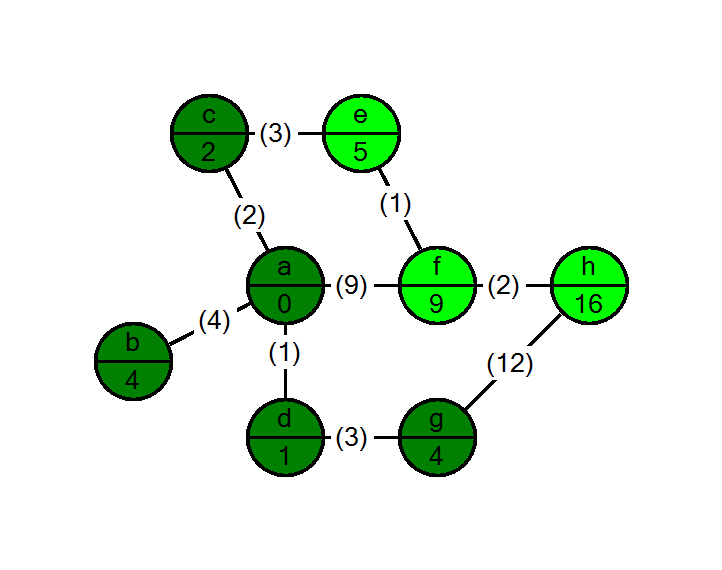
\includegraphics[width=\linewidth]{DJK/graf-djk-6}
		\caption{}
	\end{subfigure}
	\begin{subfigure}{0.32\linewidth}
		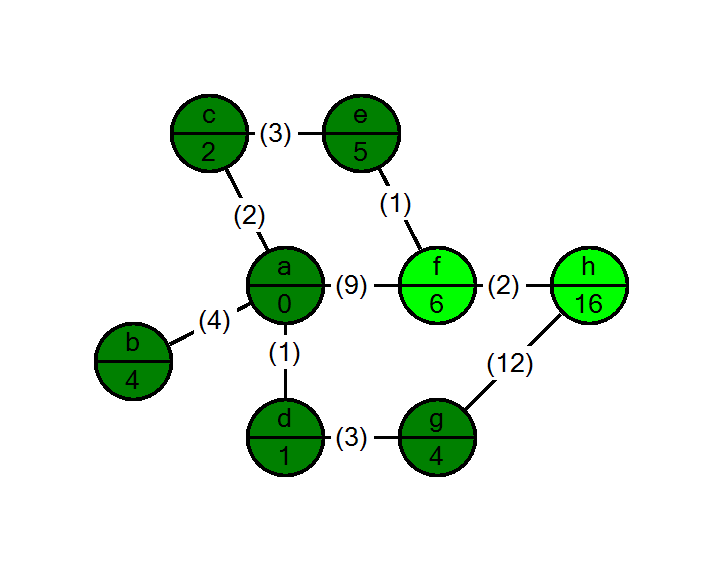
\includegraphics[width=\linewidth]{DJK/graf-djk-7}
		\caption{}
	\end{subfigure}
	\begin{subfigure}{0.32\linewidth}
		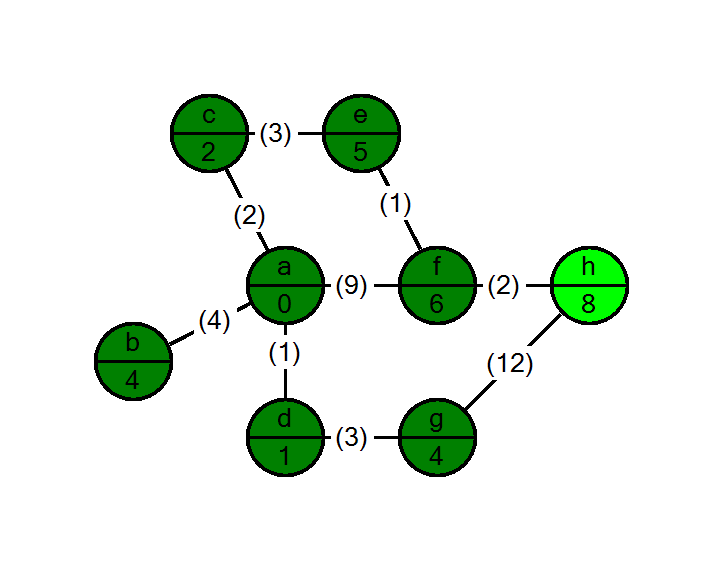
\includegraphics[width=\linewidth]{DJK/graf-djk-8}
		\caption{}
	\end{subfigure}
	\begin{subfigure}{0.32\linewidth}
		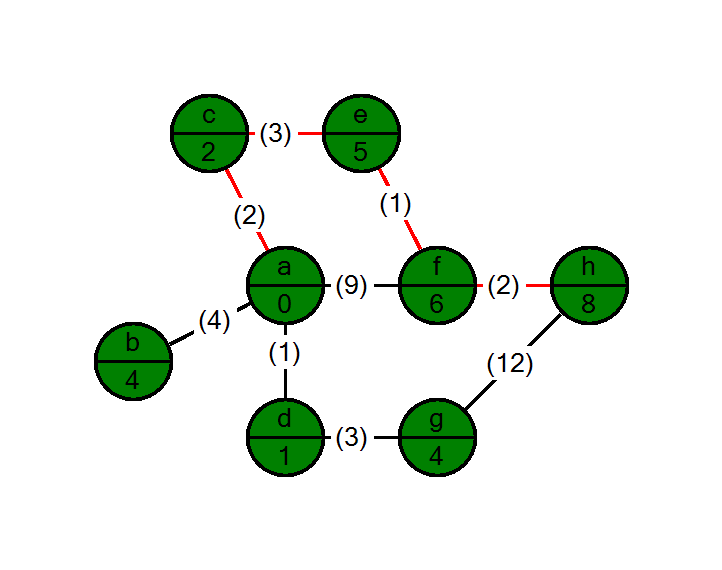
\includegraphics[width=\linewidth]{DJK/graf-djk-9}
		\caption{}
	\end{subfigure}
	\caption{Cálculo de las geodésicas entre el nodo $a$ y el nodo $h$.}
	\label{fig:djk}
\end{figure}

En la \autoref{fig:djk} se puede observar un ejemplo del algoritmo, se empieza marcando el nodo inicial, $a$, como visitado, con distancia $0$, y el resto de nodos con distancia $-1$, para señalar que no han sido visitados todavía. A continuación se escoge el nodo visitado (en verde pistacho) con menor distancia y se explora, es decir, se marcan todos sus vecinos no explorados y no visitados como visitados y se actualizan las distancias de dichos nodos como la distancia del propio nodo más el peso de la arista que los une. En caso de que un nodo vecino esté marcado como visitado, si la distancia desde el nodo actual es menor a la distancia guardada, se actualiza, como se puede observar en el apartado (g). El algoritmo termina cuando se explora el nodo final o no quedan nodos visitados que explorar. \\


Este comportamiento se puede simular utilizando una cola con prioridad en el algoritmo BFS en vez de una cola normal, de tal manera que el nodo escogido en cada paso sea el de menor distancia. \\

Se muestra a continuación el pseudocódigo asociado a la implementación del algoritmo.

\begin{breakablealgorithm}
	\caption{DJK\_geodesicas(G, v, p)}
	\begin{algorithmic}[1]
		\For{$u \in G.V$}
			\State $u.explorado = False$
			\State $u.distancia = \infty$
			\State $u.predecesor = \{\}$
		\EndFor
		\State $v.distancia = 0$
		\State $Cola\ con\ prioridad\ Q = \emptyset$
		\State $Q.push(v)$
		\While{$Q \neq \emptyset$}
			\State $u = Q.pull()$
			\If{$u == p$}
				\Return $TRUE$
			\EndIf
			\For{$n \in G.Adj[u]$}
				\If{$!n.explorado$}
					\If{$n.distancia > u.distancia + d[u][n]$}
						\State $n.distancia = u.distancia + d[u][n]$
						\State $n.predecesor = \{u\}$
						\State $Q.push(n)$
					\ElsIf{$n.distancia == u.distancia + d[u][n]$}
						\State $n.predecesor.push(u)$
					\EndIf
				\EndIf
			\EndFor
			\State $u.explorado = True$
		\EndWhile
		\Return $FALSE$
	\end{algorithmic}
\end{breakablealgorithm}

En el algoritmo anterior, $G$ es el grafo, $v$ el nodo inicial, $p$ el nodo final, $Q$ una cola con prioridad y los pesos de las aristas vienen dados en una matriz, donde el valor $d[a][b]$ corresponde al peso de la arista que une $a$ con $b$.

\section{Algoritmo de Bellman-Ford}

A continuación estudiaremos el algoritmo de Bellman-Ford, que introduce una mejora a los algoritmos anteriores al ser capaz, no sólo de funcionar con grafos con pesos negativos, si no también de detectar la existencia de ciclos negativos en un grafo, situación en la cual el camino de longitud mínima no está bien definida, pues, podríamos entrar en el ciclo negativo y reducir el coste de cualquier camino todo lo que quisiéramos. \\

Este algoritmo resuelve un problema similar al del cálculo de geodésicas entre dos nodos pero con una ligera diferencia, en este caso se calculan las geodésicas desde el nodo inicial a cualquier otro nodo del grafo. \\

Si queremos conocer las geodésicas entre dos nodos concretos, ejecutamos el algoritmo con el nodo inicial y, tras terminar, recuperamos las geodésicas a través de los padres del nodo final. \\

A partir de esta operación, el algoritmo consiste en realizar $|V|-1$ relajaciones de todas las aristas del grafo, es decir, se relajan todas las aristas del grafo y, a continuación, se repite el proceso $|V|-1$ veces. Tras esto, se comprueba la condición de relajación para cada arista, y, en caso de existir alguna arista que la cumpla, esto significa que existe un ciclo negativo y el algoritmo termina con valor $FALSE$. En caso contrario, el algoritmo termina con valor $TRUE$. \\

\begin{lema}\label{lema:corr_Bell_Ford}
	Sea $G=(V,E)$ un grafo finito con nodo inicial $s\in V$ y función de pesos $\omega : E\rightarrow \mathbb{R}$ y sea $s\in V$, suponemos además $G$ no contiene ningún ciclo negativo alcanzable desde $s$. Entonces, tras las $|V|-1$ relajaciones de todas las aristas del grafo, se tiene que $v.d = d(s,v)$ para todos los vértices alcanzables desde $s$.
\end{lema}

\begin{proof}
	Este lema se demuestra a partir de la propiedad de relajación de caminos (\autoref{lema:relaj_caminos}). Consideremos cualquier vértice $v\in V$ alcanzable desde $s$, y sea $p = v_0v_1...v_k$ con $v_0=s$ y $v_k=v$ cualquier camino de longitud mínima entre $s$ y $v$. Sabemos que este camino existe pues, como $v$ es alcanzable desde $s$, existe un camino entre ambos y, como estamos considerando un grafo finito, el número de caminos es también finito, existiendo uno con longitud mínima, que es el que buscamos. \\
	Puesto que los caminos de longitud mínima son simples, $p$ debe tener a lo sumo $|V|-1$ aristas, por lo que $k\leq|V|-1$. En cada una de las $|V|-1$ iteraciones, se relajan todas las aristas de $G$. En particular, en la $i$-ésima iteración, para $i=1,...,k$, se relaja $(v_{i-1},v_i)$. Podemos entonces aplicar la propiedad de relajación de caminos (\autoref{lema:relaj_caminos}), que nos da $v.d=v_k.d=d(s,v_k)=d(s,v)$.
\end{proof}

\begin{proposicion}
	\textbf{(Corrección del algoritmo de Bellman-Ford)} Tras aplicar el algoritmo de Bellman-Ford sobre un grafo $G=(V,E)$ finito con nodo inicial $s\in V$ y función de pesos $\omega : E\rightarrow \mathbb{R}$, si $G$ no contiene ningún ciclo negativo alcanzables desde $s$, el algoritmo devuelve $TRUE$, con $v.d=d(s,v)\ \forall v\in V$ y el subgrafo de predecesores $G_{\pi}$ es un grafo de caminos de longitud mínima con raíz $s$. Si $G$ contiene un ciclo negativo alcanzable desde $s$, entonces el algoritmo devuelve $FALSE$.
\end{proposicion}

\begin{proof}
	Supongamos primero que $G$ no contiene ningún ciclo negativo alcanzable desde $s$. Probemos primero que, tras finalizar el algoritmo, $v.d=d(s,v)\ \forall v\in V$. Si $v$ es alcanzable desde $s$, el \autoref{lema:corr_Bell_Ford} lo demuestra. Si $v$ no es alcanzable, la demostración se sigue de la propiedad de no camino (\autoref{cor:no_path}). La propiedad del subgrafo de predecesores (\autoref{prop:subg_pred}) junto al hecho probado anteriormente, implican que $G_{\pi}$ es un grafo de caminos de longitud mínima con raíz $s$. Utilizaremos a continuación el primer hecho probado para ver que el algoritmo devuelve $TRUE$, esto es, que todas las comprobaciones de la condición de relajación son falsas, es decir, $\forall (u,v)\in E,\ v.d\leq u.d+\omega(u,v)$. Para ello, basta observar que, tras terminar el algoritmo, se tiene
	\begin{align*}
		v.d & = d(s,v) \\
		& \leq d(s,u) + \omega(u,v) & (\textrm{Desigualdad triangular (\autoref{lema:des_tri})}) \\
		& = u.d + \omega(u,v)
	\end{align*}
	Por lo que el algoritmo devuelve $TRUE$. \\
	Ahora, supongamos que $G$ contiene un ciclo negativo alcanzable desde $s$, sea este ciclo $c=v_0v_1...v_k$ con $v_0=v_k$, entonces
	$$\sum_{i=1}^{k}\omega(v_{i-1},v_i)<0.$$
	Asumamos a continuación, por contradicción, que el algoritmo devuelve $TRUE$, es decir, que $v_i.d\leq v_{i-1}.d+\omega(v_{i-1},v_i)$ para $i=1,2,...,k$. Sumando dichas desigualdades, tenemos
	\begin{align*}
		\sum_{i=i}^{k}v_i.d &\leq \sum_{i=i}^{k}(v_{i-1}.d+\omega(v_{i-1},v_i)) \\
		& = \sum_{i=i}^{k}v_{i-1}.d+\sum_{i=i}^{k}\omega(v_{i-1},v_i)
	\end{align*}
	Puesto que $v_0=v_k$ cada vértice en $c$ aparece una única vez en los sumatorios $\sum_{i=i}^{k}v_i.d$ y $\sum_{i=i}^{k}v_{i-1}.d$ por lo que
	$$\sum_{i=i}^{k}v_i.d = \sum_{i=i}^{k}v_{i-1}.d.$$
	Por último, como todos los nodos del ciclo son alcanzables por $s$, se tiene que $v_i.d$ es finito para $i=1,2,...,k$, por lo que podemos cancelar los sumatorios, obteniendo
	$$\sum_{i=1}^{k}\omega(v_{i-1},v_i)\geq 0$$
	lo cuál es una contradicción, pues $c$ es un ciclo negativo. Concluimos por tanto que, en este caso, el algoritmo devuelve $FALSE$, como se quería.
\end{proof}

\subsection{Implementación del algoritmo de Bellman-Ford}

Primero se muestra una ejecución del algoritmo de Bellman-Ford sobre un grafo sencillo para ayudar al entendimiento del mismo.

\begin{figure}[htb]
	\centering
	\includegraphics[width=\linewidth]{graf-bell-ford}
	\caption{Ejecución del algoritmo de Bellman-Ford. Nodo inicial s. Los valores de $d$ aparecen dentro de cada nodo y las aristas resaltadas indica precedencia, es decir, si una arista $(u,v)$ está resaltada, significa que $u\in v.p$. Para este caso particular, el orden de relajación de aristas seguido ha sido $(t,x),(t,y),(t,z),(x,t),(y,x),(y,z),(z,x),(z,s),(s,t),(s,y)$. \textbf{(a)} indica la situación inicial tras inicializar el grafo. \textbf{(b)-(e)} indican la situación tras finalizar cada iteración de la relajación de aristas. Los valores de $d$ en (e) son los valores finales. En este caso el algoritmo devuelve $TRUE$. Esta imagen ha sido extraída de la referencia \cite{algorithms}, capítulo 24, figura 24.4.}
	\label{fig:bell-ford}
\end{figure}

El pseudocódigo asociado al algoritmo de Bellman-Ford se muestra a continuación.

\begin{breakablealgorithm}
	\caption{Bellman\_Ford(G, s)}
	\begin{algorithmic}[1]
		\State Inicializacion(G, s)
		\For{$i=1\ to |G.V|-1$}
			\For{$(u,v)\in G.E$}
				\State Relajar(u,v)
			\EndFor
		\EndFor
		\For{$(u,v)\in G.E$}
			\If{$v.d > u.d+d[u][v]$}
				\Return $FALSE$
			\EndIf
		\EndFor
		\Return $TRUE$
	\end{algorithmic}
\end{breakablealgorithm}

En el algoritmo anterior, $G$ es el grafo, $s$ el nodo inicial y los pesos de las aristas vienen dados en una matriz, donde el valor $d[a][b]$ corresponde al peso de la arista que une $a$ con $b$. \\

Las funciones $Inicializacion(G,s)$ y $Relajar(u,v)$ vienen definidas en la sección \ref{sec:2.2}.

\section{Cálculo de caminos de longitud mínima entre todas las parejas}

En esta sección se estudiarán algoritmos que resuelven el siguiente problema. \\

Dado un grafo, calcular los caminos de longitud mínima entre todas las parejas de nodos del grafo. Este problema suele aparecer en problemas como el cálculo de la distancia entre todas las ciudades dentro de un mapa, por ejemplo. \\

Podemos resolver este problema con los algoritmos descritos anteriormente, por ejemplo, ejecutando el algoritmo de Dijkstra para todo par de nodos del grafo, o ejecutando el algoritmo de Bellman-Ford desde cada nodo del grafo, en caso de tener pesos negativos, aunque esto es altamente ineficiente, por lo que en esta sección se estudiarán algoritmos específicos para este problema, más eficientes que los mencionados anteriormente. \\

En esta sección, al igual que en los algoritmos anteriores, dado el grafo $G=(V;E)$ se supondrá que los pesos de las aristas se almacenan en una matriz $d=(d_{ij})$ de orden $n\times n$ donde $|V|=n$ y

$$d_{ij}= \left\{ \begin{array}{lcc}
	0 &   si\ i=j \\
	\\ peso\ de\ la\ arista\ (i,j) &  si\ i\neq j\ y\ (i,j)\in E \\
	\\ \infty & si\ i\neq j\ y\ (i,j)\notin E
\end{array}
\right.$$

Permitimos pesos negativos, pero suponemos que los grafos no contienen ciclos negativos. La salida de los algoritmos vendrá dada por una matriz $D$ de tamaño $n\times n$ donde $d_{ij}=d(i,j)$. \\

Si, además, queremos conocer los caminos de longitud mínima entre los nodos, el algoritmo deberá calcular la matriz de predecesores $\Pi=\pi_{ij}$  donde $\pi_{ij}$ es $NULO$ si $i=j$ o no existe camino entre $i$ y $j$. En otro caso, $\pi_{ij}$ es el predecesor de $j$ en el camino de longitud mínima de $i$ a $j$. \\

A partir de esta matriz, podemos mostrar el camino de longitud mínima entre $i$ y $j$ con el siguiente algoritmo

\begin{breakablealgorithm}
	\caption{Mostrar\_Camino\_Minima\_Longitud($\Pi,i,j$)}
	\begin{algorithmic}[1]
		\If{$i==j$}
			\State $print\ i$
		\ElsIf{$\pi_{ij}==NULO$}
			\State $print\ "no\ existe\ camino\ entre\ "\ i\ "\ y\ "\ j$
		\Else
			\State Mostrar\_Camino\_Minima\_Longitud($\Pi,i,\pi_{ij}$)
		\EndIf
		\State $print\ j$
	\end{algorithmic}
\end{breakablealgorithm}

\subsection{Los caminos de longitud mínima y la multiplicación de matrices}\label{sec:3.4.1}

El primer algoritmo que veremos es recursivo y tiene cierta relación con la multiplicación de matrices, como veremos más adelante. La idea básica es construir poco a poco los caminos de longitud mínima, empezando por los que tienen una sola arista, y, a partir de estas caminos, construir los de longitud mínima con dos aristas como máximo, repitiendo este proceso hasta obtener todos los caminos de longitud mínima entre nodos. \\

Sea $l_{ij}^{(m)}$ la mínima longitud de cualquier camino entre $i$ y $j$ que contiene a lo sumo $m$ aristas. Para $m=0$ tenemos 

$$l_{ij}^{(0)}= \left\{ \begin{array}{lcc}
	0 &   si\ i=j \\
	\\ \infty & si\ i\neq j
\end{array}
\right.$$

Para $m>0$ calculamos $l_{ij}^{(m)}$ como el mínimo entre $l_{ij}^{(m-1)}$ y el mínimo de los caminos con $m$ aristas, a partir de todos los posibles predecesores $k$ de $j$. Podemos, de esta forma, definir la siguiente recursión

\begin{align*}
	l_{ij}^{(m)} & =min(l_{ij}^{(m-1)},\ min_{1\leq k\leq n}\{l_{ik}^{(m-1)}+d_{kj}\}) \\
	& =min_{1\leq k\leq n}\{l_{ik}^{(m-1)}+d_{kj}\}
\end{align*}

La última igualdad se mantiene pues $d_{jj}=0\ \forall j$. \\

Dado que todo camino de longitud mínima entre $i$ y $j$ en un grafo sin ciclos negativos es simple, contiene, a lo sumo, $n-1$ aristas, por tanto, se verifica

$$d(i,j)=l_{ij}^{(n-1)}=l_{ij}^{(n)}=l_{ij}^{(n+1)}=\dots$$.

La resolución del problema consiste, dada la recursividad anterior, en el cálculo de las matrices $L^{(1)}$, $L^{(2)}$, $L^{(3)}$, ..., $L^{(n-1)}$, donde, para $m=1,...,n-1$ tenemos $L^{(m)}=(l_{ij}^{(m)})$. Nótese que $L^{(1)}=d$ pues $l_{ij}^{(1)}=d_{ij}\forall i,j\in V$. En la \autoref{fig:3.4.1} podemos ver un ejemplo de esta recursión sobre un grafo sencillo.\\

\begin{figure}[htb]
	\centering
	\begin{subfigure}{\linewidth}
		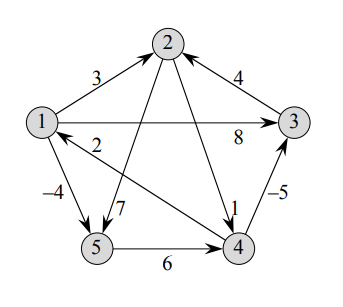
\includegraphics[width=5cm]{graf-25.1}
	\end{subfigure}

	\begin{subfigure}{\linewidth}
	$L^{(1)}=\begin{pmatrix}
		0 & 3 & 8 & \infty & -4\\
		\infty & 0 & \infty & 1 & 7 \\
		\infty & 4 & 0 & \infty & \infty \\
		2 & \infty & -5 & 0 & \infty \\
		\infty & \infty & \infty & 6 & 0
	\end{pmatrix}$
	$L^{(2)}=\begin{pmatrix}
		0 & 3 & 8 & 2 & -4\\
		3 & 0 & -4 & 1 & 7 \\
		\infty & 4 & 0 & 5 & 11 \\
		2 & -1 & -5 & 0 & -2 \\
		8 & \infty & 1 & 6 & 0
	\end{pmatrix}$
	\end{subfigure} \\
	\vspace{0.5cm}
	\begin{subfigure}{\linewidth}
	$L^{(3)}=\begin{pmatrix}
		0 & 3 & -3 & 2 & -4\\
		3 & 0 & -4 & 1 & -1 \\
		7 & 4 & 0 & 5 & 11 \\
		2 & -1 & -5 & 0 & -2 \\
		8 & 5 & 1 & 6 & 0
	\end{pmatrix}$
	$L^{(4)}=\begin{pmatrix}
		0 & 1 & -3 & 2 & -4\\
		3 & 0 & -4 & 1 & -1 \\
		7 & 4 & 0 & 5 & 3 \\
		2 & -1 & -5 & 0 & -2 \\
		8 & 5 & 1 & 6 & 0
	\end{pmatrix}$
	\end{subfigure}
	\caption{Un grafo dirigido y la sucesión de matrices $L^{(m)}$ obtenidas por el proceso recursivo definido en la sección \ref{sec:3.4.1}. La imagen del grafo ha sido extraída de la referencia \cite{algorithms}, capítulo 25, figura 25.1.}
	\label{fig:3.4.1}
\end{figure}

El corazón del algoritmo es el siguiente procedimiento, que, a partir de las matrices $L^{(m-1)}$ y $d$, calcula $L^{(m)}$.

\begin{breakablealgorithm}
	\caption{Extender\_Caminos\_Minimos($L,d$)}
	\begin{algorithmic}[1]
		\State $L'=nueva\ matriz\ n\times n$
		\For{$i=1\ hasta\ n$}
			\For{$j=1\ hasta\ n$}
				\State $l_{ij}'=\infty$
				\For{$k=1\ hasta\ n$}
					\State $l_{ij}'=min(l_{ij}',\ l_{ik}+d_{kj})$
				\EndFor
			\EndFor
		\EndFor
		\Return $L'$
	\end{algorithmic}
\end{breakablealgorithm}

El algoritmo anterior utiliza la matriz $L$ para $L^{(m-1)}$ y devuelve $L'$, que es $L^{(m)}$. \\

A partir de este procedimiento se puede ver la relación entre este algoritmo y la multiplicación de matrices. Supongamos que queremos calcular el producto matricial $C=A\cdot B$ de dos matrices de tamaño $n\times n$. Entonces, para $i,j = 1,...,n$ calcularíamos

$$c_{ij}=\sum_{k=1}^{n}a_{ik}\cdot b_{kj}$$

Realizando las sustituciones

\begin{flalign}
	l^{(m-1)} & \rightarrow a, \\
	d & \rightarrow b, \\
	l^{(m)} & \rightarrow c, \\	
	min & \rightarrow +, \\
	+ & \rightarrow .
\end{flalign}

Podemos transformar la operación de recursión en el producto matricial anterior. Gracias a este hecho, volviendo al problema del cálculo de caminos de longitud mínima, podemos calcular la matriz $L^{(n-1)}$ de la siguiente manera
\begin{adjustwidth}{5cm}{10cm}
\begin{align*}
	L^{(1)} &&=&&  d, \\
	L^{(2)} &&=&&  L^{(1)}\cdot d &&=&& & d^2,\\
	L^{(3)} &&=&&  L^{(2)}\cdot d &&=&& & d^3,\\
	&&&& \vdots \\
	L^{(m-1)} &&=&&  L^{(n-2)}\cdot d &&=&& & d^{n-1}.\\
\end{align*}
\end{adjustwidth}

Podemos calcular este proceso con el siguiente algoritmo

\begin{breakablealgorithm}
	\caption{Caminos\_Minimos\_Todas\_Parejas\_Lento($d$)}
	\begin{algorithmic}[1]
		\State $L^{(1)}=d$
		\For{$m=2\ hasta\ n-1$}
			\State $L^{(m)}=nueva\ matriz\ n\times n$
			\State $L^{(m)}=$Extender\_Caminos\_Minimos($L^{(m-1)},d$)
		\EndFor
		\Return $L^{(n-1)}$
	\end{algorithmic}
\end{breakablealgorithm}

Hemos denotado a este algoritmo como "Lento", pues podemos realizar una mejora muy sencilla que transforma el tiempo de ejecución de este último algoritmo de lineal a logarítmico. Dado que nuestro objetivo es el cálculo de la matriz $L^{(n-1)}$, no nos interesa el cálculo del resto de matrices, por ello, utilizando el hecho de que el algoritmo funciona como el producto de matrices, y que $L^{(m)}=L^{(n-1)}\ \forall m\geq n-1$, podemos calcular $L^{(n-1)}$ de la siguiente manera

\begin{adjustwidth}{3.5cm}{10cm}
	\begin{align*}
		L^{(1)} &&=&&  d, \\
		L^{(2)} &&=&&   d^2 &&=&& & d\cdot d,\\
		L^{(4)} &&=&&   d^4 &&=&&  &d^2\cdot d^2,\\
		L^{(8)} &&=&&   d^8 &&=&&  &d^4\cdot d^4,\\
		&&&& \vdots \\
		L^{(2^{\lceil lg(n-1)\rceil })} &&=&& d^{2^{\lceil lg(n-1)\rceil }} &&=&&  &d^{2^{\lceil lg(n-1)\rceil -1}}\cdot d^{2^{\lceil lg(n-1)\rceil -1}}.\\
	\end{align*}
\end{adjustwidth}

Puesto que $2^{\lceil lg(n-1)\rceil}\geq n-1$ el resultado final es igual a $L^{(n-1)}$. El siguiente algoritmo implementa dicho proceso

\begin{breakablealgorithm}
	\caption{Caminos\_Minimos\_Todas\_Parejas\_Rapido($d$)}
	\begin{algorithmic}[1]
		\State $L^{(1)}=d$
		\State $m=1$
		\While{$m<n-1$}
			\State $L^{(2m)}=nueva\ matriz\ n\times n$
			\State $L^{(2m)}=$Extender\_Caminos\_Minimos($L^{(m)},L^{(m)}$)
			\State $m=2m$
		\EndWhile
		\Return $L^{(m)}$
	\end{algorithmic}
\end{breakablealgorithm}

\subsection{Algoritmo de Floyd-Warshall}

A continuación trataremos el algoritmo de Floyd-Warshall, más eficiente que el algoritmo anterior a la hora de resolver el problema de encontrar los caminos mínimos entre todas las parejas de nodos de un grafo, para ello, el algoritmo considera los vértices intermedios en un camino de longitud mínima, siendo un vértice \textit{intermedio} de un camino simple $p=v_1...v_l$ cualquier vértice a parte de $v_1$ y $v_l$, es decir, cualquier vértice del conjunto $\{v_2,...,v_{l-1}\}$. \\

A partir de este concepto, el algoritmo de Floyd-Warshall se basa en la siguiente observación. Suponiendo que el conjunto de vértices de $G$ son $V=\{1,2,...,n\}$, consideremos un subconjunto $\{1,...,k\}$ de vértices para algún $k$. Para cualquier par de vértices $i,j\in V$ consideremos todos los caminos entre $i$ y $j$ cuyos vértices intermedios están todos en $\{1,...,k\}$, y sea $p$ un camino de longitud mínima entre ellos ($p$ es simple). El algoritmo de Floyd-Warshall utiliza una relación entre $p$ y los caminos entre $i$ y $j$ con todos los vértices intermedios están en el conjunto $\{1,...,k-1\}$. Esta relación depende del hecho de que $k$ sea un vértice intermedio de $p$ o no.

\begin{itemize}
	\item Si $k$ no es un vértice intermedio de $p$, todos los vértices intermedios están en el conjunto $\{1,...,k-1\}$. Entonces, un camino de longitud mínima desde $i$ hasta $j$ con todos los vértices intermedios están en $\{1,...,k-1\}$ es también un camino de longitud mínima desde $i$ hasta $j$ con todos los vértices intermedios en $\{1,...,k\}$.
	\item Si $k$ es un vértice intermedio en $p$, descomponemos $p$ en $i\leadsto^{p_1}k\leadsto^{p_2}j$. Por la \autoref{prop:separa_cam_min_long}, $p_1$ es un camino de longitud mínima entre $i$ y $k$ con todos los vértices intermedios en $\{1,...,k\}$. De hecho, puesto que $k$ no es un vértice intermedio, entonces $p_1$ es un camino de longitud mínima entre $i$ y $k$ con todos los vértices intermedios en $\{1,...,k-1\}$. De la forma similar, $p_2$ es un camino de longitud mínima entre $k$ y $j$ con todos los vértices intermedios en $\{1,...,k-1\}$.
\end{itemize}

A partir de esta observación, se define una fórmula recursiva al igual que se hizo anteriormente. Sea $d_{ij}^{(k)}$ el peso de un camino de longitud mínima entre $i$ y $j$ para el cuál todos sus vértices intermedios están en $\{1,...,k\}$. Cuando $k=0$, los caminos no tienen vértice intermedios, por ello, $d_{ij}^{(0)}=d_{ij}$. Definimos entonces $d_{ij}^{(k)}$ de la siguiente manera

$$d_{ij}^{(k)}= \left\{ \begin{array}{lcc}
	d_{ij} &   si\ k=0, \\
	\\ min(d_{ij}^{(k-1)},\ d_{ik}^{(k-1)}+d_{kj}^{(k-1)}) & si\ k\geq 1.
\end{array}
\right.$$

Puesto que cualquier camino tiene sus vértices intermedios en el conjunto $\{1,...,n\}$, la matriz $D^{(n)}=(d_{ij}^{(n)})$ contiene el resultado final buscado: $d_{ij}^{(n)}=d(i,j)\ \forall i,j\in V.$

\subsubsection{Implementación del algoritmo de Floyd-Warshall}

El pseudocódigo que implementa la recursión descrita anteriormente se muestra a continuación

\begin{breakablealgorithm}
	\caption{Floyd-Warshall($d$)}
	\begin{algorithmic}[1]
		\State $D^{(0)}=d$
		\For{$k=1\ hasta\ n$}
			\State $D^{(k)}=nueva\ matriz\ n\times n$
			\For{$i=1\ hasta\ n$}
				\For{$j=1\ hasta\ n$}
					\State $d_{ij}^{(k)}=min(d_{ij}^{(k-1)},\ d_{ik}^{(k-1)}+d_{kj}^{(k-1)})$
				\EndFor
			\EndFor
		\EndFor
		\Return $D^{(n)}$
	\end{algorithmic}
\end{breakablealgorithm}

Si queremos saber cuáles son los caminos de mínima longitud concretos, podemos calcular la matriz de predecesores $\Pi$ mientras se calculan las matrices $D^{(k)}$. En concreto, calculamos una secuencia de matrices $\Pi^{(0)},\Pi^{(1)},...,\Pi^{(n)}$, donde $\Pi^{(n)}=\Pi$ y $\pi_{ij}^{(k)}$ es el predecesor del vértice $j$ en un camino de longitud mínima desde $i$ con todos los vértices intermedios en el conjunto $\{1,2,...,k\}$. \\

\begin{figure}[!htb]
	\centering
	\begin{subfigure}{\linewidth}
		$D^{(0)}=\begin{pmatrix}
			0 & 3 & 8 & \infty & -4\\
			\infty & 0 & \infty & 1 & 7 \\
			\infty & 4 & 0 & \infty & \infty \\
			2 & \infty & -5 & 0 & \infty \\
			\infty & \infty & \infty & 6 & 0
		\end{pmatrix}$
		$\Pi^{(0)}=\begin{pmatrix}
			NULO & 1 & 1 & NULO & 1\\
			NULO & NULO & NULO & 2 & 2 \\
			NULO & 3 & NULO & NULO & NULO \\
			4 & NULO & 4 & NULO & NULO \\
			NULO & NULO & NULO & 5 & NULO
		\end{pmatrix}$
	\end{subfigure} \\
	\vspace{0.5cm}
	\begin{subfigure}{\linewidth}
		$D^{(1)}=\begin{pmatrix}
			0 & 3 & 8 & \infty & -4\\
			\infty & 0 & \infty & 1 & 7 \\
			\infty & 4 & 0 & \infty & \infty \\
			2 & 5 & -5 & 0 & -2 \\
			\infty & \infty & \infty & 6 & 0
		\end{pmatrix}$
		$\Pi^{(1)}=\begin{pmatrix}
			NULO & 1 & 1 & NULO & 1\\
			NULO & NULO & NULO & 2 & 2 \\
			NULO & 3 & NULO & NULO & NULO \\
			4 & 1 & 4 & NULO & 1 \\
			NULO & NULO & NULO & 5 & NULO
		\end{pmatrix}$
	\end{subfigure} \\
	\vspace{0.5cm}
	\begin{subfigure}{\linewidth}
		$D^{(2)}=\begin{pmatrix}
			0 & 3 & 8 & 4 & -4\\
			\infty & 0 & \infty & 1 & 7 \\
			\infty & 4 & 0 & 5 & 11 \\
			2 & 5 & -5 & 0 & -2 \\
			\infty & \infty & \infty & 6 & 0
		\end{pmatrix}$
		$\Pi^{(2)}=\begin{pmatrix}
			NULO & 1 & 1 & 2 & 1\\
			NULO & NULO & NULO & 2 & 2 \\
			NULO & 3 & NULO & 2 & 2 \\
			4 & 1 & 4 & NULO & 1 \\
			NULO & NULO & NULO & 5 & NULO
		\end{pmatrix}$
	\end{subfigure} \\
	\vspace{0.5cm}
	\begin{subfigure}{\linewidth}
		$D^{(3)}=\begin{pmatrix}
			0 & 3 & 8 & 4 & -4\\
			\infty & 0 & \infty & 1 & 7 \\
			\infty & 4 & 0 & 5 & 11 \\
			2 & -1 & -5 & 0 & -2 \\
			\infty & \infty & \infty & 6 & 0
		\end{pmatrix}$
		$\Pi^{(3)}=\begin{pmatrix}
			NULO & 1 & 1 & 2 & 1\\
			NULO & NULO & NULO & 2 & 2 \\
			NULO & 3 & NULO & 2 & 2 \\
			4 & 3 & 4 & NULO & 1 \\
			NULO & NULO & NULO & 5 & NULO
		\end{pmatrix}$
	\end{subfigure} \\
	\vspace{0.5cm}
	\begin{subfigure}{\linewidth}
		$D^{(4)}=\begin{pmatrix}
			0 & 3 & -1 & 4 & -4\\
			3 & 0 & -4 & 1 & -1 \\
			7 & 4 & 0 & 5 & 3 \\
			2 & -1 & -5 & 0 & -2 \\
			8 & 5 & 1 & 6 & 0
		\end{pmatrix}$
		$\Pi^{(4)}=\begin{pmatrix}
			NULO & 1 & 4 & 2 & 1\\
			4 & NULO & 4 & 2 & 1 \\
			4 & 3 & NULO & 2 & 1 \\
			4 & 3 & 4 & NULO & 1 \\
			4 & 3 & 4 & 5 & NULO
		\end{pmatrix}$
	\end{subfigure} \\
	\vspace{0.5cm}
	\begin{subfigure}{\linewidth}
		$D^{(5)}=\begin{pmatrix}
			0 & 1 & -3 & 2 & -4\\
			3 & 0 & -4 & 1 & -1 \\
			7 & 4 & 0 & 5 & 3 \\
			2 & -1 & -5 & 0 & -2 \\
			8 & 5 & 1 & 6 & 0
		\end{pmatrix}$
		$\Pi^{(5)}=\begin{pmatrix}
			NULO & 3 & 4 & 5 & 1\\
			4 & NULO & 4 & 2 & 1 \\
			4 & 3 & NULO & 2 & 1 \\
			4 & 3 & 4 & NULO & 1 \\
			4 & 3 & 4 & 5 & NULO
		\end{pmatrix}$
	\end{subfigure} \\
	\caption{Secuencia de matrices $D^{(k)}$ y $\Pi^{(k)}$ obtenida a partir del algoritmo de Floyd-Warshall aplicado al grafo de la figura \autoref{fig:3.4.1}}
	\label{fig:3.4.2}
\end{figure}

Para $k=0$, como no hay vértices intermedios, tenemos

$$\pi_{ij}^{(0)}= \left\{ \begin{array}{lcc}
	NULO &   si\ i=j\ o\ d_{ij}=\infty, \\
	\\ i & si\ i\neq j\ y\ d_{ij}<\infty.
\end{array}
\right.$$

Para $k\geq 1$, si al introducir el vértice $k$ hemos creado un camino de longitud menor, escogemos el predecesor de $j$ en un camino de longitud mínima desde $k$, calculado en la iteración $k-1$, si no, nos quedamos con el mismo predecesor que la iteración anterior. Formalmente, 

$$\pi_{ij}^{(k)}= \left\{ \begin{array}{lcc}
	\pi_{ij}^{(k-1)} &   si\ d_{ij}^{(k-1)}\leq d_{ik}^{(k-1)}+d_{kj}^{(k-1)}, \\
	\\ \pi_{kj}^{(k-1)} &   si\ d_{ij}^{(k-1)}> d_{ik}^{(k-1)}+d_{kj}^{(k-1)}.
\end{array}
\right.$$

En la \autoref{fig:3.4.2} podemos observar el resultado de la ejecución del algoritmo sobre un grafo simple. \\

A continuación se muestra el pseudocódigo completo del algoritmo, incluyendo la construcción de la matriz de predecesores

\begin{breakablealgorithm}
	\caption{Floyd-Warshall-Caminos($G,d$)}
	\begin{algorithmic}[1]
		\State $D^{(0)}=d$
		\State $\Pi^{(0)}=nueva\ matriz\ nula\ n\times n$
		\For{$(i,j)\in G.E$}
			\State $\pi_{ij}^{(0)}=i$
		\EndFor
		\For{$k=1\ hasta\ n$}
			\State $D^{(k)},\Pi^{(k)}=nueva\ matriz\ n\times n$
			\For{$i=1\ hasta\ n$}
				\For{$j=1\ hasta\ n$}
					\If{$d_{ij}^{(k-1)}\leq d_{ik}^{(k-1)}+d_{kj}^{(k-1)}$}
						\State $d_{ij}^{(k)}=d_{ij}^{(k-1)}$
						\State $\pi_{ij}^{(k)}=\pi_{ij}^{(k-1)}$
					\Else
						\State $d_{ij}^{(k)}=d_{ik}^{(k-1)}+d_{kj}^{(k-1)}$
						\State $\pi_{ij}^{(k)}=\pi_{kj}^{(k-1)}$
					\EndIf
				\EndFor
			\EndFor
		\EndFor
		\Return $(D^{(n)},\Pi^{(n)})$
	\end{algorithmic}
\end{breakablealgorithm}

\subsubsection{Clausura transitiva de un grafo dirigido}

\begin{definicion}
	Dado un grafo dirigido $G=(V,E)$, se define la \textit{clausura transitiva} de $G$ como el grafo $G^*=(V,E^*)$, donde
	$$E^*=\{(i,j):\ existe\ un\ camino\ desde\ i\ hasta\ j\}.$$
\end{definicion}

La clausura transitiva de un grafo dirigido es muy útil, pues nos permite saber de forma rápida si existe un camino entre dos nodos o no. Para calcularla, basta con asignar peso $1$ a todas las aristas del grafo y ejecutar el algoritmo de FLoyd-Warshall. \\

\begin{figure}[htb]
	\centering
	\begin{subfigure}{\linewidth}
		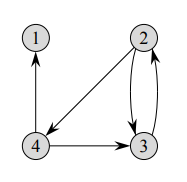
\includegraphics[width=3.5cm]{graf-clausura-transitiva}
	\end{subfigure}
	
	\begin{subfigure}{\linewidth}
		$T^{(0)}=\begin{pmatrix}
			1 & 0 & 0 & 0 &\\
			0 & 1 & 1 & 1 \\
			0 & 1 & 1 & 0 \\
			1 & 0 & 1 & 1 \\
		\end{pmatrix}$
		$T^{(1)}=\begin{pmatrix}
			1 & 0 & 0 & 0 &\\
			0 & 1 & 1 & 1 \\
			0 & 1 & 1 & 0 \\
			1 & 0 & 1 & 1 \\
		\end{pmatrix}$
		$T^{(2)}=\begin{pmatrix}
			1 & 0 & 0 & 0 &\\
			0 & 1 & 1 & 1 \\
			0 & 1 & 1 & 1 \\
			1 & 0 & 1 & 1 \\
		\end{pmatrix}$
	\end{subfigure} \\
	\vspace{0.5cm}
	\begin{subfigure}{\linewidth}
		$T^{(3)}=\begin{pmatrix}
			1 & 0 & 0 & 0 &\\
			0 & 1 & 1 & 1 \\
			0 & 1 & 1 & 1 \\
			1 & 1 & 1 & 1 \\
		\end{pmatrix}$
		$T^{(4)}=\begin{pmatrix}
			1 & 0 & 0 & 0 &\\
			1 & 1 & 1 & 1 \\
			1 & 1 & 1 & 1 \\
			1 & 1 & 1 & 1 \\
		\end{pmatrix}$
	\end{subfigure}
	\caption{Un grafo dirigido y las matrices $T^{(k)}$ calculadas por el algoritmo de la clausura transitiva. La imagen del grafo ha sido extraída de la referencia \cite{algorithms}, capítulo 25, figura 25.5.}
	\label{fig:claus-trans}
\end{figure}

Además, puesto que no necesitamos calcular ningún valor numérico para la clausura transitiva, podemos sustituir los valores numéricos del algoritmo por valores booleanos, es decir, que sólo pueden tomar el valor $0$ ($FALSE$) o $1$ ($TRUE$) y sustituir la operaciones aritméticas por operaciones lógicas. De esta forma podemos ahorrar tiempo y espacio, puesto que las operaciones lógicas son generalmente más rápidas y los valores booleanos ocupan menos espacio. \\

En particular, para aplicar estos cambios, definimos $t_{ij}^{(k)}$ como $1$ si existe un camino entre $i$ y $j$ con vértices intermedios en $\{1,...,k\}$ y $0$ en otro caso. De esta manera podemos construir la clausura transitiva $G^*=(V,E^*)$ añadiendo una arista $(i,j)$ a $E^*$ si $t_{ij}^{(n)}=1$. Para calcular $t_{ij}^{(k)}$ se sigue la siguiente recursión

$$t_{ij}^{(0)}= \left\{ \begin{array}{lcc}
	0 &   si\ i\neq j\ y\ (i,j)\notin E, \\
	\\ 1 & si\ i= j\ o\ (i,j)\in E,
\end{array}
\right.$$

y para $k\geq 1$,

$$t_{ij}^{(k)}=t_{ij}^{(k-1)}\lor (t_{ik}^{(k-1)}\wedge t_{kj}^{(k-1)}).$$ \\

El psuedocódigo que implementa este algoritmo es el siguiente

\begin{breakablealgorithm}
	\caption{Clausura\_Transitiva($G,d$)}
	\begin{algorithmic}[1]
		\State $T^{(0)}=nueva\ matriz\ nula\ n\times n$
		\For{$i=1\ hasta\ n$}
			\For{$j=1\ hasta\ n$}
				\If{$i==j\ or\ (i,j)\in G.E$}
					\State $t_{ij}^{(0)}=1$
				\EndIf
			\EndFor
		\EndFor
		\For{$k=1\ hasta\ n$}
			\State $T^{(k)}=nueva\ matriz\ n\times n$
			\For{$i=1\ hasta\ n$}
				\For{$j=1\ hasta\ n$}
					\State $t_{ij}^{(k)}=t_{ij}^{(k-1)}\lor (t_{ik}^{(k-1)}\wedge t_{kj}^{(k-1)})$
				\EndFor
			\EndFor
		\EndFor
		\Return $T^{(n)}$
	\end{algorithmic}
\end{breakablealgorithm}

Para ilustrar este proceso, en la \autoref{fig:claus-trans} se puede observar el cálculo de las matrices $T^{(k)}$ sobre un grafo arbitrario.



\endinput





% !TeX root = ../libro.tex
% !TeX encoding = utf8

\setchapterpreamble[c][0.75\linewidth]{%
	\sffamily
	Una vez hemos construido un algoritmo correcto, un paso importante es determinar su costo computacional, es decir, los recursos que necesita, tales como el tiempo o espacio. El análisis necesario para estimar estos costes es un problema teórico, para el cuál requeriremos de un marco formal, que definiremos al principio de este capítulo. \\
	Además veremos los costes de los algoritmos estudiados en el \autoref{ch:tercer-capitulo}. \\
	\par\bigskip
}
\chapter{Complejidad algorítmica}\label{ch:cuarto-capitulo}

Como ya mencionamos anteriormente, necesitamos un marco formal para estudiar la complejidad de un algoritmo, por ello utilizaremos la notación asintótica, que introducimos con las siguientes definiciones.

\begin{definicion}
	Dadas dos funciones $f,g:\mathbb{N}\rightarrow \mathbb{R}$ diremos que $f(n)=\Theta(g(n))$ si existen constantes $c_1,c_2$ y $n_0$ tales que $$0\leq c_1g(n)\leq f(n)\leq c_2g(n)\ \ \ \forall n\geq n_0.$$
\end{definicion}

\begin{definicion}
	Dadas dos funciones $f,g:\mathbb{N}\rightarrow \mathbb{R}$ diremos que $f(n)=O(g(n))$ si existen constantes $c$ y $n_0$ tales que $$0\leq f(n)\leq cg(n)\ \ \ \forall n\geq n_0.$$
\end{definicion}

\begin{definicion}
	Dadas dos funciones $f,g:\mathbb{N}\rightarrow \mathbb{R}$ diremos que $f(n)=\Omega(g(n))$ si existen constantes $c$ y $n_0$ tales que $$0\leq cg(n)\leq f(n)\ \ \ \forall n\geq n_0.$$
\end{definicion}

En esencia, la idea es establecer una cota para el crecimiento asintótico de una función a partir de otra, normalmente más simple. En particular, la notación $\Omega$ implica una cota inferior, $O$ una cota superior y $\Theta$ ambas. En la \autoref{fig:notacion_asintotica} podemos observar un ejemplo de cada tipo de notación. \\

\begin{figure}[!htb]
	\centering
	\begin{subfigure}{\linewidth}
		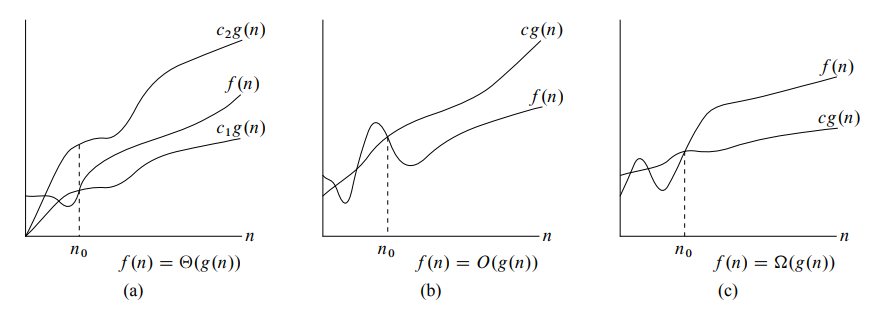
\includegraphics[width=14cm]{notacion_asintotica}
	\end{subfigure}
	
	\caption{Ejemplos gráficos de las notaciones $\Theta,O$ y $\Omega$. En cada imagen se muestra el valor mínimo para $n_0$, pero cualquier valor superior funciona también. Para el caso \textbf{(a)}, la notación $\Theta(g(n))$ implica una cota superior e inferior, por lo que la gráfica de $f(n)$ debe situarse entre las cotas obtenidas a partir de $g(n)$ y las constantes $c_1$ y $c_2$. En \textbf{(b)}, la notación $O(g(n))$ establece una cota superior, por lo que la gráfica de $f(n)$ se debe situar por debajo de la cota, obtenida a partir de la constante $c$. Por último, en \textbf{(c)} la notación $\Omega$ implica una cota inferior, luego en este caso, la gráfica de $f(n)$ debe de estar por encima de dicha cota, obtenida a partir de $c$. La imagen ha sido extraída de la referencia \cite{algorithms}, capítulo 3, figura 3.1.}
	\label{fig:notacion_asintotica}
\end{figure}

Utilizaremos la notación asintótica principalmente para describir el tiempo de ejecución de los algoritmos, pues es el recurso más importante, normalmente. Aunque también se suele estudiar el costo en espacio del algoritmo. \\

Cuando hablamos de tiempo de ejecución, hay que especificar de qué tiempo estamos hablando exactamente, pues existen varios interesantes. Entre otros, el tiempo medio de ejecución, el del peor caso, o el del mejor. Normalmente los datos más interesantes son el tiempo medio, pues es el tiempo de ejecución medio del algoritmo, y el tiempo de ejecución del peor caso, que establece un límite al tiempo máximo de ejecución del algoritmo. \\

Para poder analizar el tiempo de ejecución de un algoritmo de manera formal, tenemos que establecer un modelo de computación. En nuestro caso, supondremos que el computador tarda exactamente una unidad de tiempo en realizar cualquier instrucción básica, como pueden ser la suma, asignación, comparación, etc. Además, tomaremos como variables para medir el tiempo el tamaño del grafo de entrada, en concreto, el número de nodos y aristas. De esta manera, si decimos que un algoritmo es de orden $O(V)$ para un grafo $G=(V,E)$, nos referimos a que es lineal en el número de nodos. \\

A la hora de analizar los algoritmos estudiados, debemos tener en cuenta que en una cola normal, las operaciones \textbf{push()} y \textbf{pull()} son de orden $O(1)$, mientras que en una cola con prioridad, la operación \textbf{push()} es de orden $O(log(n))$ donde $n$ es el tamaño de la cola, y \textbf{pull()} es de orden $O(1)$. Nótese que estos órdenes son específicos para la librería estándar de C++ y podrían variar para otro lenguaje.

\section{Búsqueda en anchura}

Empezaremos por el algoritmo de Búsqueda en anchura (\autoref{BFS}). Primero tenemos que, debido a que cada vez que exploramos un nodo, lo marcamos como tal, y comprobamos que un nodo no haya sido explorado antes de proceder, las operaciones con la cola son de orden $O(V)$. Además, como itera sobre la lista de adyacencia de cada nodo sólo cuando es explorado, el algoritmo recorre cada lista de adyacencia una única vez. Como la suma de las longitudes de todas las listas de adyacencia es $\Theta(E)$, el tiempo gastado en escanear las listas es de $O(E)$. Por último, como el bucle de inicialización recorre una vez cada nodo, es de orden $O(V)$. Tenemos, en definitiva, que el algoritmo de búsqueda en anchura es de orden $O(V+E)$. Es decir, es lineal en el tamaño de la representación mediante listas de adyacencia de $G$.

\section{Dijkstra}

Continuamos con el algoritmo de Dijkstra (\autoref{DJK}). El análisis de este algoritmo es en esencia el mismo que el realizado para el algoritmo de búsqueda en anchura, pues la base del algoritmo es la misma. La única diferencia es el hecho de que utiliza colas con prioridad. Por esto, dado que la operación \textbf{push()} es de orden $O(log(V))$, y que esta operación se realiza dentro de los dos bucles principales del procedimiento, el orden final del algoritmo de Dijkstra es $O((V+E)log(V))$.

\section{Bellman-Ford}

Seguimos con el algoritmo de Bellman-Ford (\autoref{Bellman-Ford}). En este caso, el análisis es bastante simple, al ser un algoritmo muy corto. Primero, la operación de relajación es de orden $O(1)$, pues consta de comprobaciones y asignaciones. Ahora, por orden, la inicialización del algoritmo recorre todos los nodos del grafo, luego es de orden $O(V)$. A continuación tenemos dos bucles anidados, el primero recorre todos los nodos menos uno, y el segundo, por cada nodo, recorre todas las aristas. Este proceso es, por tanto, de orden $O(VE)$. El último bucle recorre todas las aristas realizando una comprobación, por lo que es de orden $O(E)$. En definitiva, el algoritmo de Bellman-Ford es de orden $O(VE)$.

\section{Algoritmo asociado a la multiplicación de matrices}

Analizaremos a continuación las dos versiones descritas en la \autoref{sec:3.4.1} asociadas a la multiplicación de matrices. Primero, el procedimiento $Extender_Caminos_Minimos(L,d)$, consta de tres bucles anidados, que realizan $n$ iteraciones cada uno, siendo $n$ el tamaño de la matriz de adyacencia, es decir, el número de nodos. El procedimiento es, por tanto, de orden $O(V^3)$. Ahora, la versión "Lenta" del algoritmo realiza este procedimiento dentro de un bucle una cantidad total de $n-2$ veces, luego es de orden $O(V)$, teniendo entonces un orden de $O(V^4)$ para la versión "Lenta" del algoritmo. La versión "Rápida" del algoritmo realiza el procedimiento $log_2(n)$ veces, gracias a los cálculos realizados en la descripción del algoritmo, siendo, por tanto, de orden $O(V^3log(V))$.

\section{Algoritmo de Floyd-Warshall}

Por último analizaremos la complejidad del algoritmo de Floyd-Warshall (\autoref{Floyd-Warshall}). Primero, el algoritmo base de Floyd-Warshall, que consta de tres bucles anidados que realizan cada uno $n$ iteraciones, siendo $n$ el tamaño de la matriz de adyacencia, es decir, el número de nodos. Puesto que las únicas operaciones que realiza el algoritmo son las de asignación, creación de matrices y la llamada a la función $min()$, todas de orden $O(1)$, el algoritmo es de orden $O(V^3)$. \\

El algoritmo completo, que calcula además los caminos, es idéntico en la parte de los tres bucles anidados, la única diferencia es que la operación de asignación donde se llamaba a la función $min()$, se ha sustituido por el condicional equivalente, que también es de orden $O(1)$. La parte que añade esta versión es la inicialización de la matriz $\Pi^(0)$, para la cuál se recorren todas las aristas del grafo. El orden del algoritmo es, por tanto, $O(V^3 + E) = O(V^3)$. Esta última igual es debida a que el número máximo de aristas en un grafo es $V(V-1)$, y, claramente, $V(V-1)<V^3$. \\

El algoritmo de la clausura transitiva tiene la misma estructura que la versión completa del algoritmo de Floyd-Warshall, luego es también de orden $O(V^3)$, aunque hay que destacar que el uso de variables booleanas hace que sea más rápido que el algoritmo principal.

\endinput





% !TeX root = ../libro.tex
% !TeX encoding = utf8

\setchapterpreamble[c][0.75\linewidth]{%
	\sffamily
	En este capítulo abordaremos los detalles más importantes de la implementación realizada en C++ de los algoritmos. Así como el cálculo de tiempos de ejecución para comparar con la complejidad teórica calculada en el \autoref{ch:cuarto-capitulo}. Para mostrar los tiempos de ejecución y los ajustes a las funciones de complejidad se utilizará Gnuplot \cite{alma991008609239704990}.
	\par\bigskip
}
\chapter{Experimentación}\label{ch:quinto-capitulo}

Toda la implementación está disponible en el siguiente repositorio de \href{https://github.com/PabloC01/TFG}{GitHub}\footnote{Dirección url: https://github.com/PabloC$01$/TFG}. La implementación se encuentra en la carpeta \textit{Codigo}, dividida a su vez en $4$ carpetas:

\begin{itemize}
	\item \textit{FUENTES}: contiene los archivos fuente con el propio código y el archivo \textit{MAKEFILE}.
	\item \textit{Grafos}: contiene archivos con la representación de los grafos que se muestran a lo largo de la sección 3.
	\item \textit{Resultados}: contiene los archivos de texto con los tiempos de ejecución obtenidos.
	\item \textit{bin}: contiene los programas ejecutable, así como el script de cálculo de tiempos y un archivo de texto \textit{LEEME} con instrucciones.
\end{itemize}

Para representar las estructuras necesarias para implementar los algoritmos se han utilizado los TDA más comunes de la STL de C++ \cite{alma991014010751904990}, como pueden ser la clase \textit{vector<>} o \textit{queue<>}, en función de las necesidades requeridas por las diferentes estructuras a implementar.

\section{Clase Grafo}

Utilizaremos esta clase para poder representar grafos en C++. Está implementada en los archivos \textit{Grafos.h} y \textit{Grafos.cpp}, en ellos se implementa la propia clase, que consiste de una matriz que se utilizará como matriz de adyacencia, otra matriz que se utilizará como lista de adyacencia y otras variables asociadas al grafo como el número de nodos. Además se implementa una función para construir la lista de adyacencia a partir de la matriz de adyacencia, para poder construir los grafos de manera más simple. \\

También se implementan dos funciones para generar grafos de forma aleatoria, para ello simplemente generamos aristas aleatorias hasta llenar el número de aristas del grafo, que se calculan de la siguiente manera a partir de la densidad del grafo:

$$|E| = |V|(|V| - 1)d$$

donde $d$ es la densidad del grafo, representada como número decimal, entre $0$ y $1$. \\

Como parte de la clase \textit{Grafo} se incluyen también constructores para poder guardar un grafo a partir de la matriz de adyacencia y atributos del grafo. También se ha implementado un constructor para guardar un grafo a partir de un archivo de texto, donde aparezcan primero los atributos del grafo y, depués, la matriz de adyacencica. Por último se incluye una función para mostrar la matriz de adyacencia del grafo y el número de nodos.

\section{Búsqueda en anchura}

Los dos algoritmos de Búsqueda en anchura están implementado en los archivos \textit{BFS.h} y \textit{BFS.cpp}. Por comodidad, se han utilizado dos vectores de la STL para guardar la distancia actual de un nodo y si ha sido explorado o no. No se han incluido estos atributos a la clase \textit{Grafo} para hacerla lo más simple posible, pues no todos los algoritmos utilizan estos atributos. \\

A parte de esto, como ya se comentó anteriormente, se ha utilizado el TDA \textit{queue<>} para simular la Cola en el algoritmo de búsqueda en anchura. Por último se ha utilizado la constante \textit{INT\_MAX} para simular el infinito.

\section{Dijkstra}

El algoritmo de Dijkstra está implementado en los archivos \textit{DJK.h} y \textit{DJK.cpp}. La implementación es igual a la búsqueda en anchura, salvo por el uso de la cola con prioridad. Para implementar dicha cola se ha utilizado el TDA \textit{priority\_queue<>}, creando para ello una clase \textit{comparador}, que compare dos nodos en función de su distancia actual almacenada en el vector de distancias.

\section{Bellman-Ford}

El algoritmo de Bellman-Ford está implementado en los archivos \textit{BF.h} y \textit{BF.cpp}. Por simplificar el código se ha incluido el código del proceso de relajación de una arista directamente al cuerpo del algoritmo, pues es el único algoritmo que utiliza dicho proceso. \\

A la hora de crear el vector de distancias, en este caso, en vez de utilizar la constante \textit{INT\_MAX}, se le ha restado una catidad arbitrariamente grande, pero bastante más pequeña que dicha constante. Esto es por un simple motivo, el condicional en la operación de relajación suma la distancia actual con el peso de la arista que se está relajando. En el caso de que la distancia actual sea \textit{INT\_MAX}, si le sumamos el peso, produce overflow, convirtiéndose en un número negativo, y, por tanto, rompiendo el algoritmo. Esto nunca sucede sin embargo en los dos algoritmos anteriores porque dicha comprobación sólo se realiza sobre nodos que han salido de la Cola, y a dichos nodos siempre se le modifica la distancia actual por una menor que \textit{INT\_MAX}.

\section{Multiplicación de matrices y Floyd-Warshall}

Estos algoritmos están implementados en los archivos \textit{Warshall.h} y \textit{Warshall.cpp}. La implementación de estos algoritmos ha sido algo más problemática y complicada que el resto. Principalmente debido a que la aritmética con el infinito hay que simularla mediante el uso de constantes y condicionales para separar casos en los que las variables son ``infinitas'' o no. \\

Además hay que construir la matriz inicial, pues partimos de la matriz de adyacencia, que no tiene los valores infinitos, necesarios para el funcionamiento de los algoritmos. \\

Los algoritmos de Floyd-Warshall y la Clausura Transitiva por otro lado han sido más sencillos de implementar, sin ningún contratiempo importante.

\section{Programas principales}

Se han creado dos programas principales, \textit{TFG.cpp} y \textit{Tiempos.cpp}. El primero ejecuta todos los algoritmos y muestra los resultados sobre un grafo aleatorio o un grafo almacenado en un archivo de texto. El segundo muestra el tiempo de ejecución del algoritmo pasado como parámetro, repitiendo la ejecución $10$ veces y calculando la media. \\

A continuación se muestra la salida del programa principal para cada algoritmo sobre el ejemplo con el que se explicó cada algoritmo.

\subsection{Resultado BFS}

\begin{figure}[!htb]
	\centering
	\begin{subfigure}{\linewidth}
		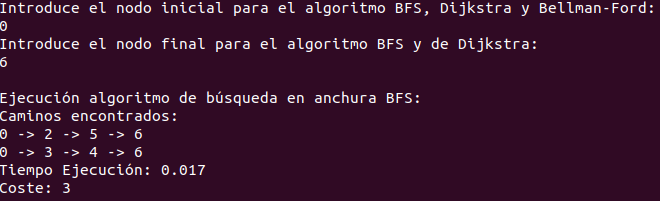
\includegraphics[width=14cm]{./Tiempos_Ejecucion/Ejecucion_BFS}
	\end{subfigure}
	
	\caption{Resultado de ejecución del algoritmo BFS con el grafo de la \autoref{fig:bfs-camino}.}
	\label{fig:resultado_BFS}
\end{figure}

\subsection{Resultado BFS Conexas}

\begin{figure}[!htb]
	\centering
	\begin{subfigure}{\linewidth}
		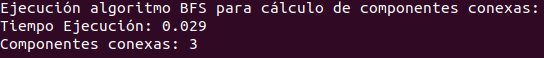
\includegraphics[width=12cm]{./Tiempos_Ejecucion/Ejecucion_BFS_C}
	\end{subfigure}
	
	\caption{Resultado de ejecución del algoritmo BFS Conexas con el grafo de la \autoref{fig:bfs-conexas}.}
	\label{fig:resultado_BFS_C}
\end{figure}

\subsection{Resultado Dijkstra}

Para este ejemplo los nodos $a$-$h$ son los nodos $0$-$7$ por lo que el camino obtenido se traduce como $a - c - e - f - h$.

\begin{figure}[!htb]
	\centering
	\begin{subfigure}{\linewidth}
		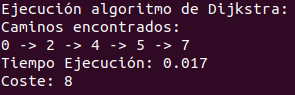
\includegraphics[width=6cm]{./Tiempos_Ejecucion/Ejecucion_DJK}
	\end{subfigure}
	
	\caption{Resultado de ejecución del algoritmo DJK con el grafo de la \autoref{fig:djk}.}
	\label{fig:resultado_DJK}
\end{figure}

\subsection{Resultado Bellman-Ford}

En este caso la numeración es la siguiente: $s:0$, $t:1$, $y:2$, $x:3$, $z:4$.

\begin{figure}[!htb]
	\centering
	\begin{subfigure}{\linewidth}
		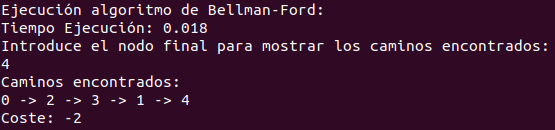
\includegraphics[width=12cm]{./Tiempos_Ejecucion/Ejecucion_BF}
	\end{subfigure}
	
	\caption{Resultado de ejecución del algoritmo BF con el grafo de la \autoref{fig:bell-ford}.}
	\label{fig:resultado_BF}
\end{figure}

\subsection{Resultado algoritmos de multiplicación de matrices}

\begin{figure}[!htb]
	\centering
	\begin{subfigure}{\linewidth}
		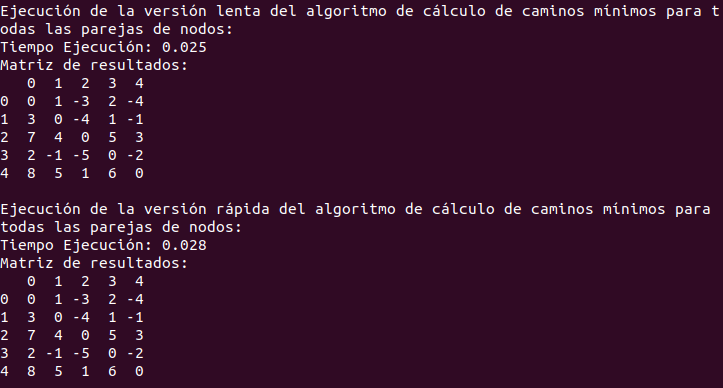
\includegraphics[width=12cm]{./Tiempos_Ejecucion/Ejecucion_Matrices}
	\end{subfigure}
	
	\caption{Resultado de ejecución de los algoritmos de multiplicación de matrices con el grafo de la \autoref{fig:3.4.1}.}
	\label{fig:resultado_Matrices}
\end{figure}

\newpage

\subsection{Resultado Floyd-Warshall}

En este caso se muestra además el camino encontrado entre el nodo $0$ y $1$, construido a partir de la matriz de predecesores.

\begin{figure}[!htb]
	\centering
	\begin{subfigure}{\linewidth}
		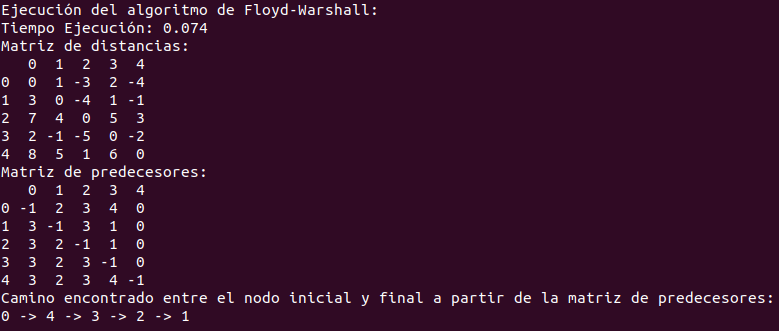
\includegraphics[width=12cm]{./Tiempos_Ejecucion/Ejecucion_FW}
	\end{subfigure}
	
	\caption{Resultado de ejecución del algoritmo de FW con el grafo de la \autoref{fig:3.4.1}.}
	\label{fig:resultado_FW}
\end{figure}

\subsection{Resultado clausura transitiva}

\begin{figure}[!htb]
	\centering
	\begin{subfigure}{\linewidth}
		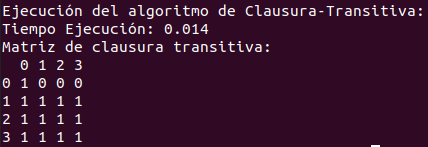
\includegraphics[width=12cm]{./Tiempos_Ejecucion/Ejecucion_CT}
	\end{subfigure}
	
	\caption{Resultado de ejecución del algoritmo de la clausura transitiva con el grafo de la \autoref{fig:claus-trans}.}
	\label{fig:resultado_CT}
\end{figure}

\section{Medición de tiempos y comparación con la complejidad teórica}

Para calcular el tiempo de ejecución de los algoritmos, utilizamos la función \textit{clock()} de C++, que devuelve el número de \textit{ticks} transcurridos desde una época relativa a la ejecución del programa. Ejecutando dicha función antes y después de llamar a la función que implementa el algoritmo y calculando la diferencia conseguimos el tiempo de ejecución. En este caso se ha medido en milisegundos. \\

Ya hemos comentado cómo se extraen los tiempos de un algoritmo concreto a partir del programa principal \textit{Tiempos.cpp}. Para extraer los tiempos de todos los algoritmos, se ha programado un script de bash, llamado \textit{calculo\_tiempos.sh}, situado en la carpeta \textit{bin}. Dicho script ejecuta y guarda en un archivo los tiempos de ejecución de cada algoritmo para $10$ números de nodos distintos, incrementándolos en cada ejecución. \\

Otro detalle importante es cómo medir el tamaño, pues tenemos dos cantidades, $|V|$ y $|E|$, y para ajustar la complejidad, necesitamos que la función dependa de una única variable. Para ello, utilizamos la densidad para escribir el número de aristas en función del número de vértices, y escogemos una densidad fija para calcular todos los tiempos. En este caso se ha escogido una desidad de $0.1$, aunque no tiene mucha importancia el número en concreto. \\

Una vez obtenidos los tiempos, que se guardan en la carpeta \textit{Resultados}, podemos mostrarlos utilizando la función \textit{plot} de Gnuplot. Las figuras \autoref{fig:tiempos_BFS} - \autoref{fig:tiempos_Todos} muestran las gráficas obtenidas mediante esta función, que representan los tiempos de ejecución de cada algoritmo en milisegundos en función del número de vértices. \\

\begin{figure}[!htb]
	\centering
	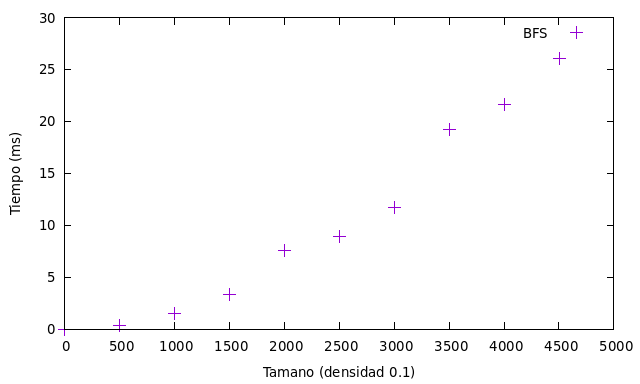
\includegraphics[width=9cm]{./Tiempos_Ejecucion/Tiempos_BFS_0.1}
	
	\caption{Tiempos de ejecución BFS.}
	\label{fig:tiempos_BFS}
\end{figure}

\begin{figure}[!htb]
	\centering
	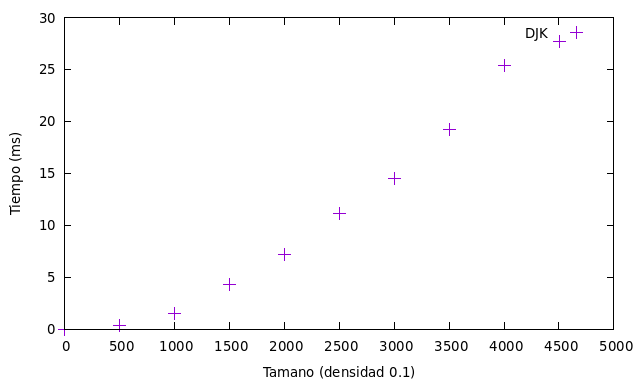
\includegraphics[width=9cm]{./Tiempos_Ejecucion/Tiempos_DJK_0.1}
	
	\caption{Tiempos de ejecución Dijkstra.}
	\label{fig:tiempos_DJK}
\end{figure}

\begin{figure}[!htb]
	\centering
	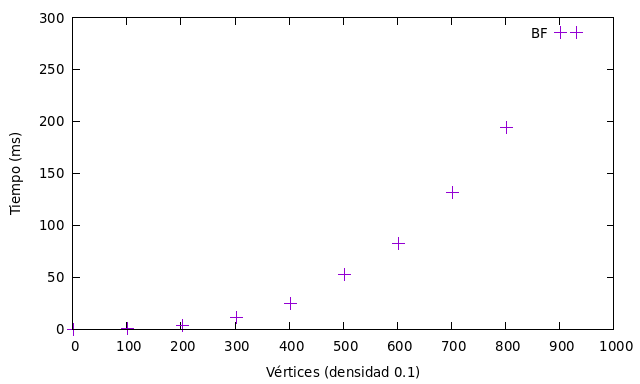
\includegraphics[width=9cm]{./Tiempos_Ejecucion/Tiempos_BF}
	
	\caption{Tiempos de ejecución Bellman-Ford.}
	\label{fig:tiempos_BF}
\end{figure}

\begin{figure}[!htb]
	\centering
	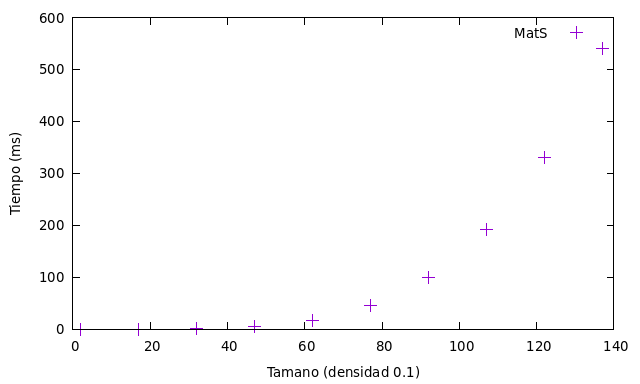
\includegraphics[width=9cm]{./Tiempos_Ejecucion/Tiempos_MatS}
	
	\caption{Tiempos de ejecución algoritmo de matrices lento.}
	\label{fig:tiempos_MatS}
\end{figure}

\begin{figure}[!htb]
	\centering
	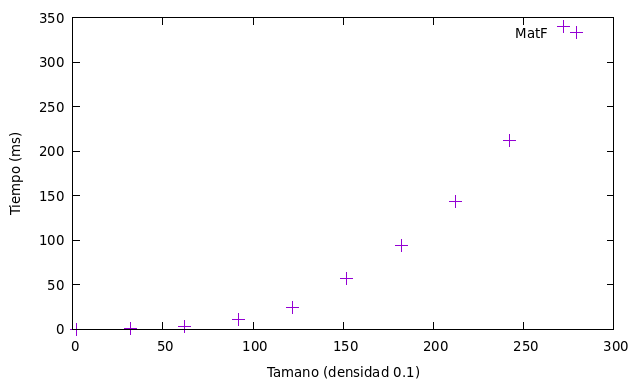
\includegraphics[width=9cm]{./Tiempos_Ejecucion/Tiempos_MatF}
	
	\caption{Tiempos de ejecución algoritmo de matrices rápido.}
	\label{fig:tiempos_MatF}
\end{figure}

\begin{figure}[!htb]
	\centering
	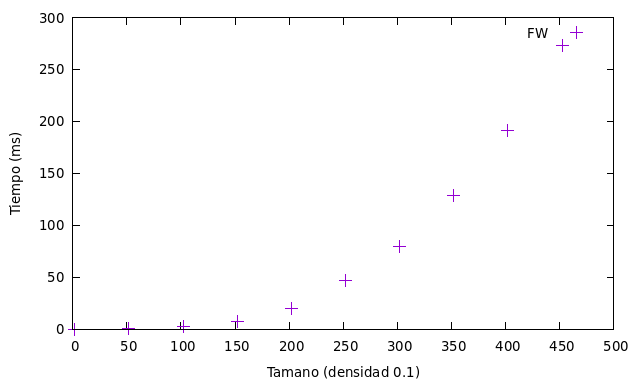
\includegraphics[width=9cm]{./Tiempos_Ejecucion/Tiempos_FW}
	
	\caption{Tiempos de ejecución Floyd-Warshall.}
	\label{fig:tiempos_FW}
\end{figure}

\begin{figure}[!htb]
	\centering
	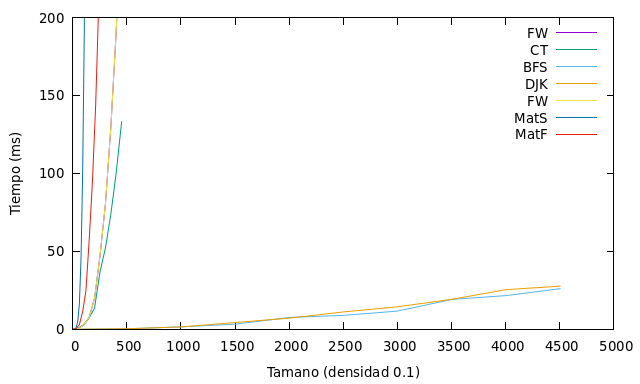
\includegraphics[width=9cm]{./Tiempos_Ejecucion/Tiempos_Todos}
	
	\caption{Tiempos de ejecución de todos los algoritmos.}
	\label{fig:tiempos_Todos}
\end{figure}

\subsection{Tiempo de ejecución de los algoritmos BFS y Dijkstra}

\begin{figure}[htb]
	\centering
	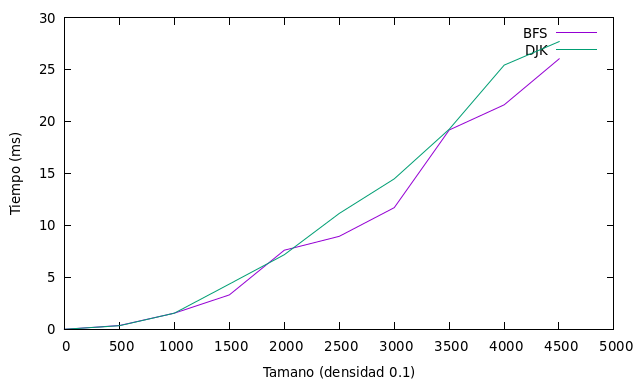
\includegraphics[width=7cm]{./Tiempos_Ejecucion/Tiempos_BFS_DJK_0.1}
	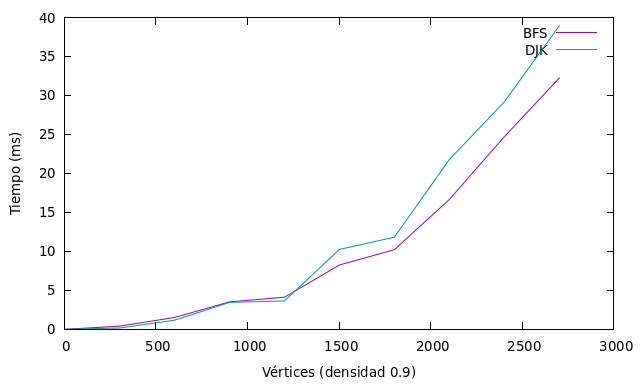
\includegraphics[width=7cm]{./Tiempos_Ejecucion/Tiempos_BFS_DJK_0.9}
	
	\caption{Comparación entre los tiempos de ejecución del algoritmo BFS y Dijkstra para distintas densidades de grafos.}
	\label{fig:BFS_DJK}
\end{figure}

En este apartado vamos a comentar un curioso resultado obtenido tras probar con diferentes densidades de grafos. Si observamos la implementación del algoritmo de Dijkstra, la única diferencia con BFS es el uso de la cola con prioridad, cuya operación de inserción tiene complejidad igual al logaritmo del tamaño de la cola. Esto hace que, sobre grafos dispersos, como la cola no suele estar muy llena, esta operación sea relativamente rápida, consiguiendo por tanto tiempos muy similares a BFS, esta diferencia se puede apreciar en las gráficas de la \autoref{fig:BFS_DJK} , donde se han extraído tiempos para densidades de grafo de $0.1$ y $0.9$.

\subsection{Tiempo de ejecución de los algoritmos Floyd-Warshal y de clausura transitiva}

Mostramos aquí la comparación entre los tiempos de ejecución del algoritmo de Floyd-Warshall y la clausura transitiva, para comprobar como, efectivamente, el uso de variables booleanas y funciones lógicas es menos costoso en tiempo, para ello en la \autoref{fig:FW_CT} mostramos un gráfico con los tiempos de ejecución de ambos algoritmos.

\begin{figure}[htb]
	\centering
	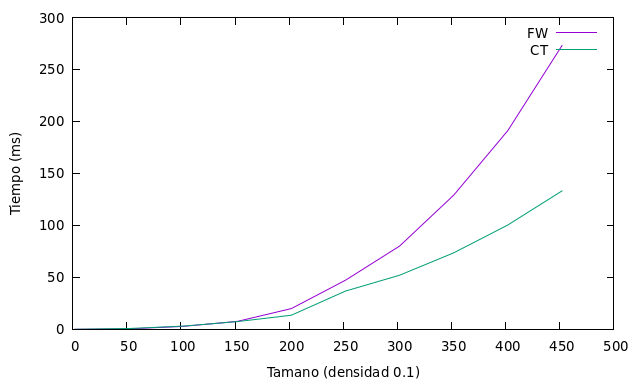
\includegraphics[width=7cm]{./Tiempos_Ejecucion/Tiempos_FW_CT}
	
	\caption{Comparación entre los tiempos de ejecución del algoritmo de Floyd-Warshall y la clausura transitiva.}
	\label{fig:FW_CT}
\end{figure}

\subsection{Contraste con la complejidad teórica}

Para llevar a cabo este contraste se ha utilizado la función \textit{fit} de Gnuplot, que ajusta una función creada a una serie de puntos. El proceso a seguir es simple, se crea una función que represente la complejidad teórica y se ajusta a los resultados obtenidos. Si la función ajusta bien los resultados obtenidos, entonces podemos concluir que la complejidad teórica es correcta. \\

La función a crear depende de la complejidad, por ejemplo, si la complejidad es $O(V^2)$, la función a ajustar sería $f(x) = a_0x^2 + a_1$. Ya hemos comentado que escribimos el número de aristas en función del número de vértices. Por ello, en el caso de ser complejidad $O(E)$, por ejemplo, la función sería $f(x) = a_0x(x-1)0.1 + a_1$, pues la densidad la hemos fijado a $0.1$. \\ 

En las figuras \autoref{fig:ajuste_BFS} - \autoref{fig:ajuste_FW} se pueden ver las gráficas de las funciones ajustadas superpuestas con los tiempos de ejecución junto a la función ajustada y la complejidad teórica. Se puede observar como todas las complejidades son correctas.\\

\newpage

Complejidad: $O(V+E)$, función: $f(x) = a_0x + a_1x(x-1)0.1 + a_2$

\begin{figure}[!htb]
	\centering
	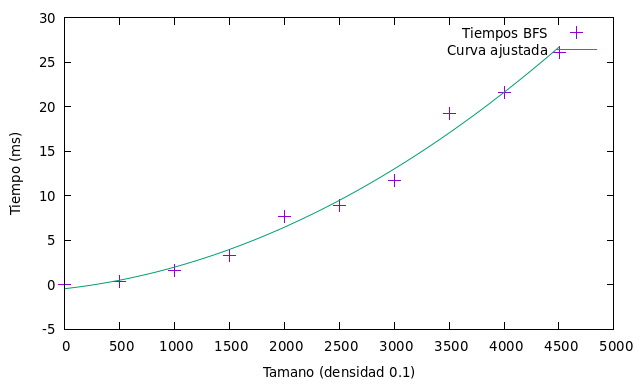
\includegraphics[width=8.5cm]{./Tiempos_Ejecucion/Ajuste_BFS}
	
	\caption{Ajuste de la complejidad del algoritmo BFS.}
	\label{fig:ajuste_BFS}
\end{figure}


Complejidad: $O((V+E)log(V))$, función: $f(x) = (a_0x + a_1x(x-1)0.1)a_2log(x) + a_3$

\begin{figure}[!htb]
	\centering
	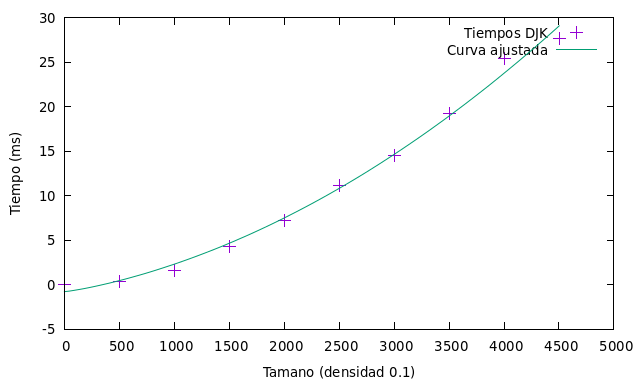
\includegraphics[width=8.5cm]{./Tiempos_Ejecucion/Ajuste_DJK}
	
	\caption{Ajuste de la complejidad del algoritmo de Dijkstra.}
	\label{fig:ajuste_DJK}
\end{figure}


Complejidad: $O(VE)$, función: $f(x) = a_0xa_1x(x-1)0.1 + a_2$

\begin{figure}[!htb]
	\centering
	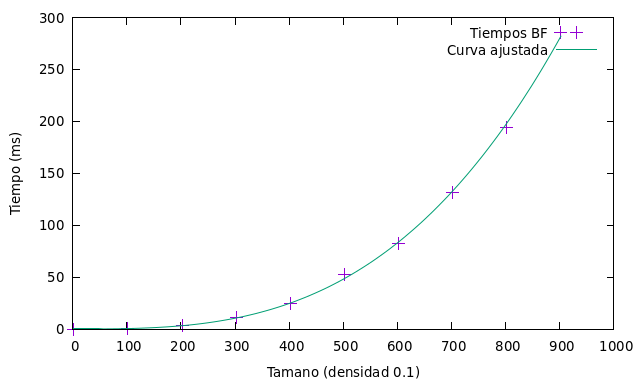
\includegraphics[width=8.5cm]{./Tiempos_Ejecucion/Ajuste_BF}
	
	\caption{Ajuste de la complejidad del algoritmo de Bellman-Ford.}
	\label{fig:ajuste_BF}
\end{figure}

\newpage

Complejidad: $O(V^4)$, función: $f(x) = a_0x^4 + a_1$

\begin{figure}[!htb]
	\centering
	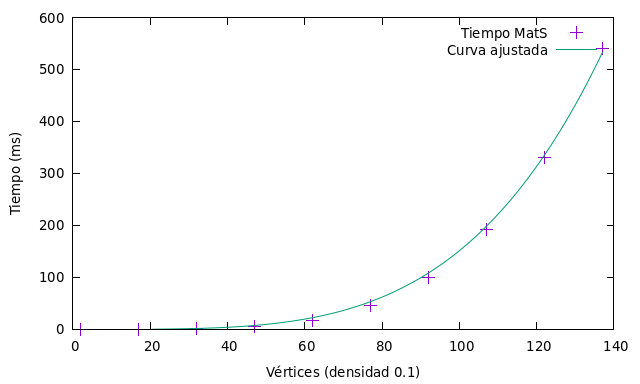
\includegraphics[width=8.5cm]{./Tiempos_Ejecucion/Ajuste_MatS}
	
	\caption{Ajuste de la complejidad del algoritmo de matrices lento.}
	\label{fig:ajuste_MatS}
\end{figure}

Complejidad: $O(V^3log(V))$, función: $f(x) = a_0x^3 + a_1log(x) + a_2$

\begin{figure}[!htb]
	\centering
	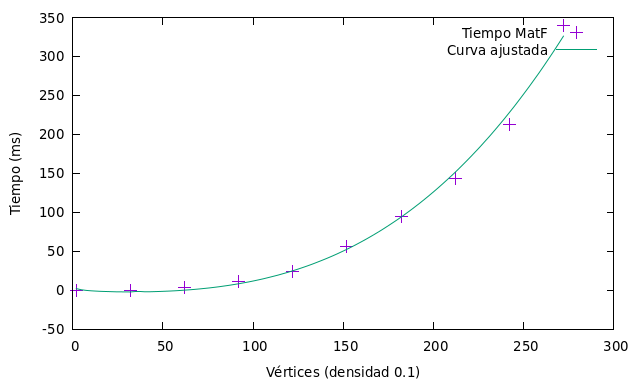
\includegraphics[width=8.5cm]{./Tiempos_Ejecucion/Ajuste_MatF}
	
	\caption{Ajuste de la complejidad del algoritmo de matrices rápido.}
	\label{fig:ajuste_MatF}
\end{figure}

Complejidad: $O(V^3)$, función: $f(x) = a_0x^3 + a_1$

\begin{figure}[!htb]
	\centering
	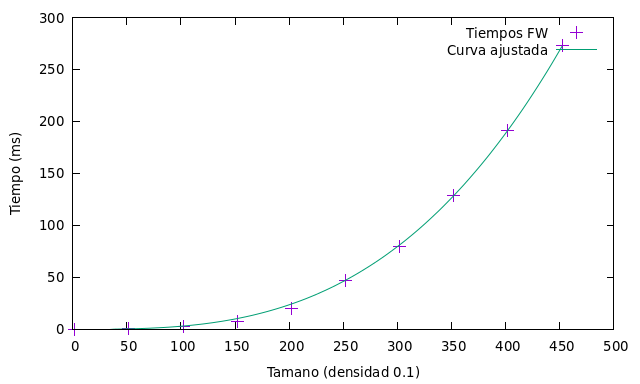
\includegraphics[width=8.5cm]{./Tiempos_Ejecucion/Ajuste_FW}
	
	\caption{Ajuste de la complejidad del algoritmo de Floyd-Warshall.}
	\label{fig:ajuste_FW}
\end{figure}

\endinput





% !TeX root = ../libro.tex
% !TeX encoding = utf8

\setchapterpreamble[c][0.75\linewidth]{%
	\sffamily
	En este capítulo comentaremos las conclusiones obtenidas en este trabajo además de hablar sobre posibles trabajos futuros que puedan surgir a raíz de este trabajo.
	\par\bigskip
}
\chapter{Conclusiones y trabajos futuros.}\label{ch:sexto-capitulo}

\section{Conclusiones}

En este trabajo se ha abordado el problema del cálculo de geodésicas sobre un grafo, un problema para el cual se han propuesto muchas soluciones, dependiendo sobre todo de las características del grafo de entrada, si es dirigido, ponderado, con pesos negativos, etc. Hemos estudiado los algoritmos principales que existen para resolver este problema para cada tipo de grafo. \\

Para grafos no ponderados, los más simples, el algoritmo de búsqueda en anchura, para grafos ponderados con pesos positivos, el algoritmo de Dijsktra y, para cualquier grafo en general, el algoritmo de Bellman-Ford. Además de explorar el problema del cálculo de geodésicas entre dos nodos fijos, se ha estudiado también el problema de encontrar las geodésicas entre cualquier par de nodos del grafo. Problema que hemos resuelto con el algoritmo de Floyd-Warshall. \\

Se han utilizado los conocimientos adquiridos a lo largo de la carrera, no sólo de la parte de matemáticas para poder entender y describir la base sobre grafos necesaria para la realización del trabajo. Sino también de la parte de informática, para poder entender, describir e implementar todos los algoritmos estudiados en el trabajo. Que incluye tanto la propia implementación de los algoritmos como la generación de archivos con tiempos de ejecución. Además de la compilación de todos los archivos mediante el uso de la herramienta \textit{make}. \\

Además se ha estudiado la complejidad teórica de los algoritmos, y se ha comprobado que la implementación de los algoritmos efectivamente tienen la complejidad teórica calculada.

\section{Trabajos Futuros}

Este trabajo es tan solo una introducción al cálculo de geodésicas sobre grafos, existen gran diversidad de algoritmos que no hemos estudiado en este trabajo. Como por ejemplo el algoritmo de Prim \cite{6773228} o el algoritmo de Kruskall \cite{fc0df122-3305-33a8-bac5-7a6fc3666dfb}. Se podría por tanto continuar con la investigación analizando otros algoritmos. \\

Además, los cambios introducidos en este trabajo al algoritmo de búsqueda en anchura, Dijkstra y Bellman-Ford para que calculen todas las geodésicas en vez de una sola abre la posibilidad al estudio de aplicaciones reales en las que estas variantes aporten una cierta utilidad que no aportan las versiones clásicas. \\

Este trabajo se puede ampliar también escogiendo uno o varios problemas de la vida real relacionados con el cálculo de caminos de mínima longitud sobre grafos y aplicarles los algoritmos implementados para resolverlos. \\

También se puede profundizar más en la implementación de los algoritmos, mejorando la eficiencia de los mismos. Algo para lo cuál el lenguaje escogido, C++, es perfecto. \\

Por último está la posibilidad de intentar desarrollar un nuevo algoritmo, por ejemplo, centrándose en un problema real e intentando mejorar la eficiencia de los algoritmos ya existentes.

\endinput





% --------------------------------------------------------------------
% APPENDIX: Opcional
% --------------------------------------------------------------------

\appendix % Reinicia la numeración de los capítulos y usa letras para numerarlos
\pdfbookmark[-1]{Apéndices}{appendix} % Alternativamente podemos agrupar los apéndices con un nuevo \part{Apéndices}

% !TeX root = ../libro.tex
% !TeX encoding = utf8

\chapter{Primer apéndice}\label{ap:apendice1}

\section{Ejemplo extendido de cálculo de geodésicas con BFS}

Con afán de mostrar el procedimiento del algoritmo BFS sobre un grafo de mayor extensión, se presenta a continuación en la \autoref{fig:bfs-camino-big} el proceso de búsqueda de geodésicas, donde cada imagen representa el estado del grafo al finalizar una capa, es decir, tras explorar por completo cada bola, el nodo inicial es el nodo $0$, y el nodo final está marcado en rojo para mejor visibilidad. Los nodos ya explorados se han marcado en verde oscuro, y los nodos visitados pero no explorados, es decir, los nodos en la cola, en verde pistacho. Los caminos marcados en rojo representan las geodésicas encontradas, que se pueden calcular a través de los predecesores de cada nodo.

\begin{figure}[htb]
	\centering
	\begin{subfigure}{0.28\linewidth}
		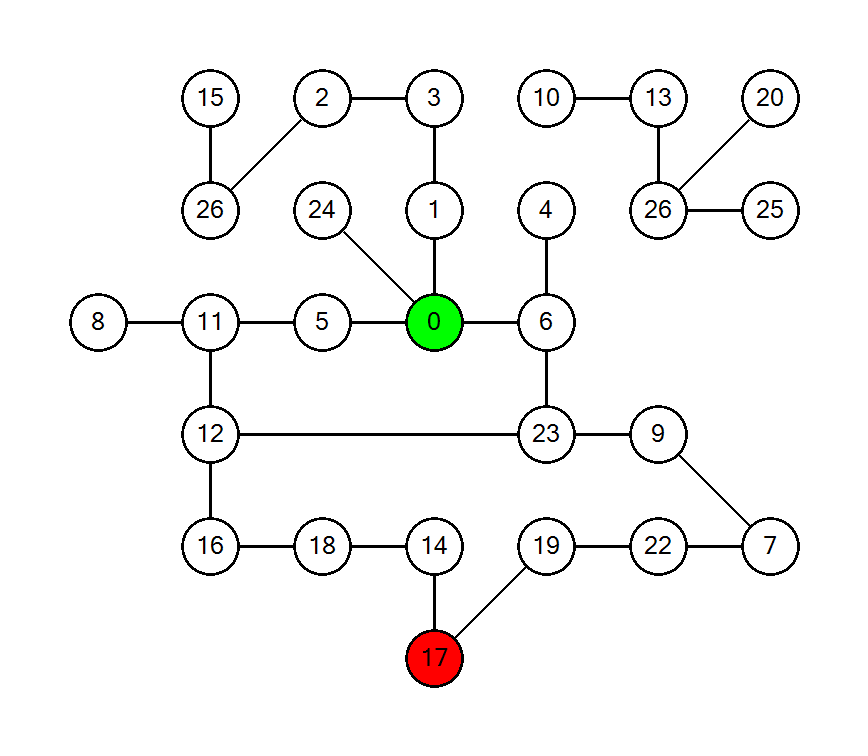
\includegraphics[width=\linewidth]{BFS/graf-bfs-camino-big-1}
		\caption{}
	\end{subfigure}
	\begin{subfigure}{0.28\linewidth}
		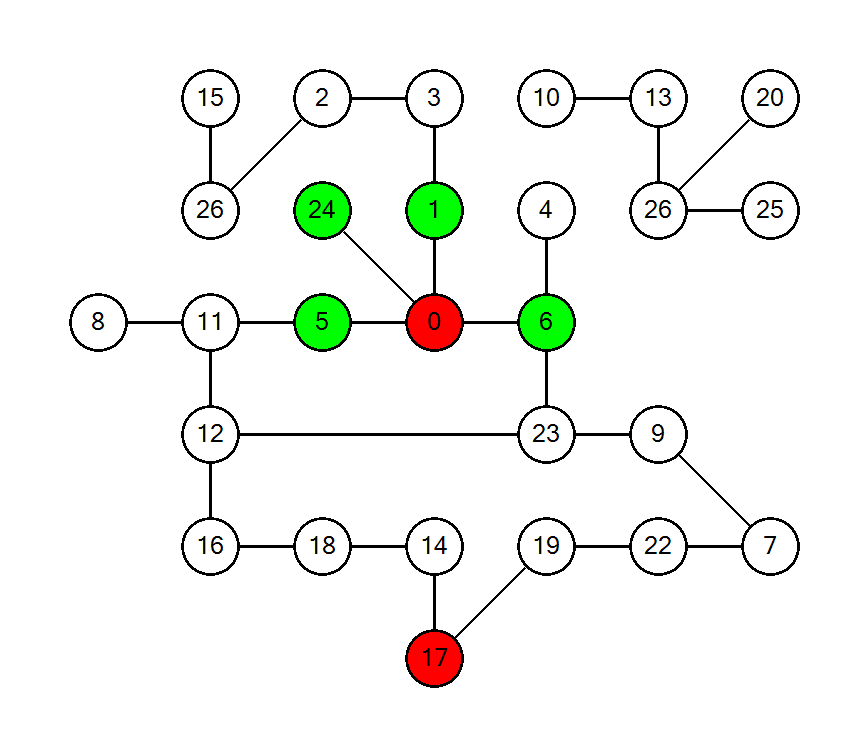
\includegraphics[width=\linewidth]{BFS/graf-bfs-camino-big-2}
		\caption{}
	\end{subfigure}
	\begin{subfigure}{0.28\linewidth}
		\includegraphics[width=\linewidth]{BFS/graf-bfs-camino-big-3}
		\caption{}
	\end{subfigure}
	\begin{subfigure}{0.28\linewidth}
		\includegraphics[width=\linewidth]{BFS/graf-bfs-camino-big-4}
		\caption{}
	\end{subfigure}
	\begin{subfigure}{0.28\linewidth}
		\includegraphics[width=\linewidth]{BFS/graf-bfs-camino-big-5}
		\caption{}
	\end{subfigure}
	\begin{subfigure}{0.28\linewidth}
		\includegraphics[width=\linewidth]{BFS/graf-bfs-camino-big-6}
		\caption{}
	\end{subfigure}
	\begin{subfigure}{0.28\linewidth}
		\includegraphics[width=\linewidth]{BFS/graf-bfs-camino-big-7}
		\caption{}
	\end{subfigure}
	\begin{subfigure}{0.28\linewidth}
		\includegraphics[width=\linewidth]{BFS/graf-bfs-camino-big-8}
		\caption{}
	\end{subfigure}
	\begin{subfigure}{0.28\linewidth}
		\includegraphics[width=\linewidth]{BFS/graf-bfs-camino-big-9}
		\caption{}
	\end{subfigure}
	\caption{Cálculo de las geodésicas entre el nodo $0$ y el nodo $17$, marcado en rojo.}
	\label{fig:bfs-camino-big}
\end{figure}


\endinput
%------------------------------------------------------------------------------------
% FIN DEL APÉNDICE. 
%------------------------------------------------------------------------------------

% !TeX root = ../libro.tex
% !TeX encoding = utf8

\chapter{Estimación de costes}\label{ap:apendice2}

Como parte de este trabajo se presenta a continuación una estimación detallada de los posibles costes que acarrean el presente trabajo. Establecemos un precio por hora de $30$€. Dividiremos el trabajo en $3$ aspectos:

\begin{itemize}
	\item Estudio teórico de la teoría de grafos necesaria para la formalización de los algoritmos.
	\item Estudio de los algoritmos que se analizarán al lo largo del trabajo.
	\item Implementación de los algoritmos y obtención de resultados.
	\item Composición de la memoria.
\end{itemize}

En la \autoref{tb:tabla-costes} se puede observar el desglose comentado.

\begin{table}[htpb]
	\centering
	\begin{tabular}{lrr} \toprule
		\textbf{Concepto} & \textbf{Cantidad(horas)} & \textbf{Coste total (€)}          \\ \toprule
		Estudio de conceptos básicos sobre la teoría de grafos & 30 & 900          \\ 
		Estudio de propiedades sobre caminos de mínima longitud & 20 & 600          \\ \bottomrule
		Algoritmo BFS & 10 & 300          \\ 
		Algoritmo de Dijkstra & 10 & 300          \\
		Algoritmo de Bellman-Ford & 20 & 600          \\ 
		Algoritmo de Floyd-Warshall & 20 & 600          \\
		Estudio de la complejidad algorítmica & 10 & 300          \\  \bottomrule
		Implementación del código fuente & 40 & 1200 \\ 
		Obtención de resultados & 10 & 300 \\ \bottomrule
		Redacción de la memoria & 60 & 1800          \\ 
		Correcciones & 15 & 450          \\ \bottomrule
		\textbf{Total} & \textbf{245} & \textbf{7350}          \\ \bottomrule
	\end{tabular}
	\caption{Tabla de costes}
	\label{tb:tabla-costes}
\end{table}

\endinput
%------------------------------------------------------------------------------------
% FIN DEL APÉNDICE. 
%------------------------------------------------------------------------------------

% Añadir tantos apéndices como sea necesario 

% --------------------------------------------------------------------
% GLOSARIO: Opcional
% --------------------------------------------------------------------

% !TeX root = ../libro.tex
% !TeX encoding = utf8

\chapter*{Glosario}
\addcontentsline{toc}{chapter}{Glosario} % Añade el glosario a la tabla de contenidos

La inclusión de un glosario es opcional.

Archivo: \texttt{glosario.tex}

\begin{description} 
  \item[$\mathbb{R}$] Conjunto de números reales.

  \item[$\mathbb{C}$] Conjunto de números complejos.

  \item[$\mathbb{Z}$] Conjunto de números enteros.
\end{description}
\endinput
 

% -------------------------------------------------------------------
% BACKMATTER
% -------------------------------------------------------------------

\backmatter % Desactiva la numeración de los capítulos
\pdfbookmark[-1]{Referencias e Índices}{BM-Referencias}

% BIBLIOGRAFÍA
%-------------------------------------------------------------------

\setbibpreamble{Las referencias se listan por orden alfabético. Aquellas referencias con más de un autor están ordenadas de acuerdo con el primer autor.\par\bigskip}
\bibliographystyle{alpha} 
\begin{small} % Normalmente la bibliografía se imprime en un tamaño de letra más pequeño.
\bibliography{library.bib}
\end{small}


% ÍNDICE TERMINOLÓGICO  (Opcional) 
%------------------------------------------------------------------- 

% Para incluir el índice terminológico es necesario descomentar los siguientes comandos. Incluir un índice terminológico es opcional

% \cleardoublepage 
% \begin{footnotesize} % Normalmente el índice se imprime en un tamaño de letra más pequeño.
% \printindex 
% \end{footnotesize}

\end{document}
